\section{Section 2 - Gaussian convolution implemented via FFT}

\subsection{Question 14}

\begin{minipage}{\linewidth}
  \begin{minipage}{0.4\linewidth}
    \begin{figure}[H]
    	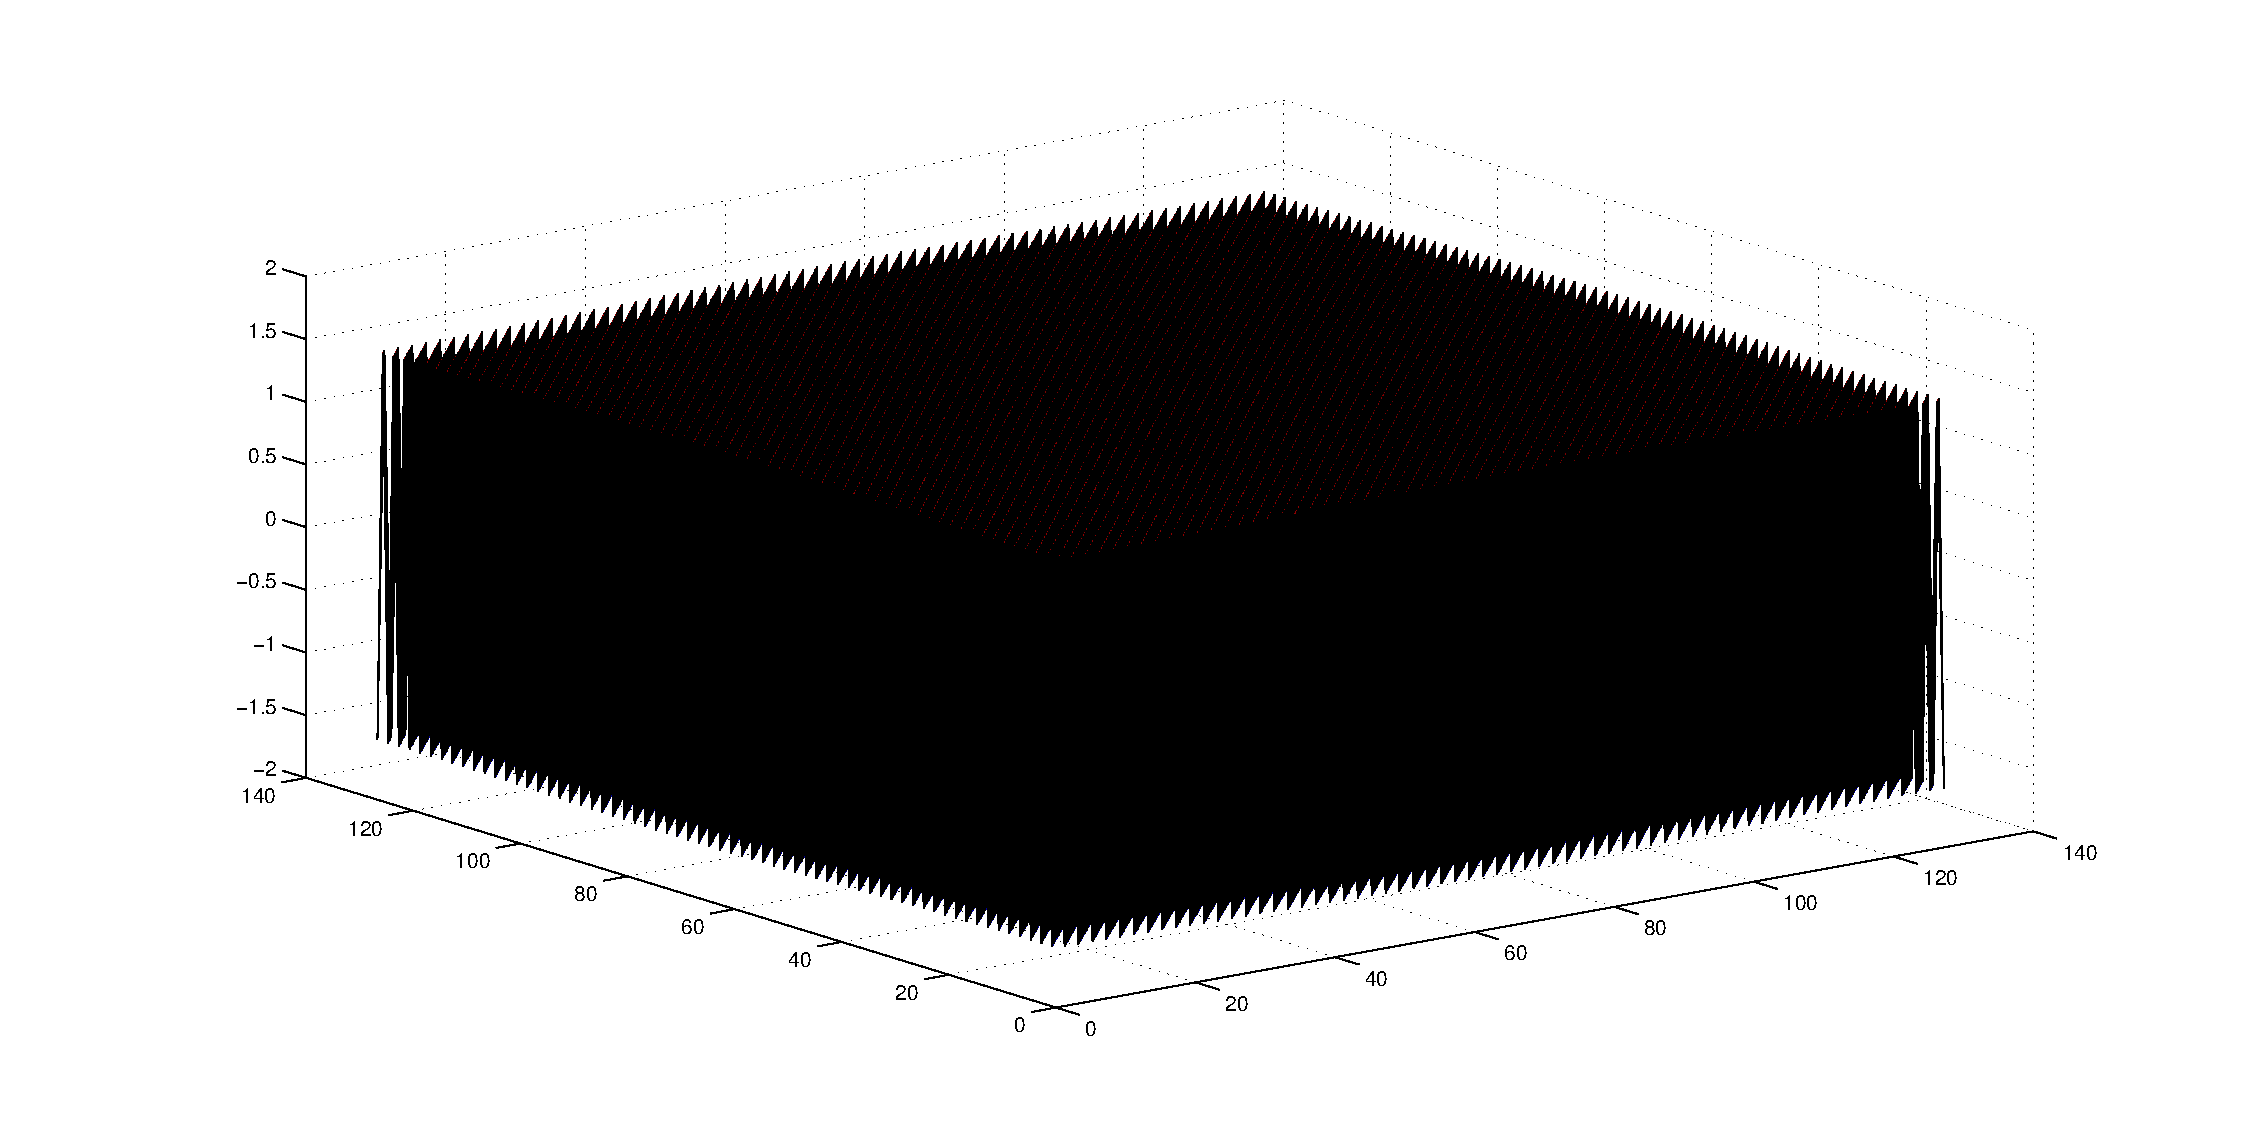
\includegraphics[scale=0.2]{./images/Q14/t01.eps}
      	\caption{Impulse response of the discretized $g(m,n;\ t)$ for $t=0.1$.}
      	\label{fig:Q14_t01}
    \end{figure}
  \end{minipage}
  \hspace{0.05\linewidth}
  \begin{minipage}{0.4\linewidth}
    \begin{figure}[H]
        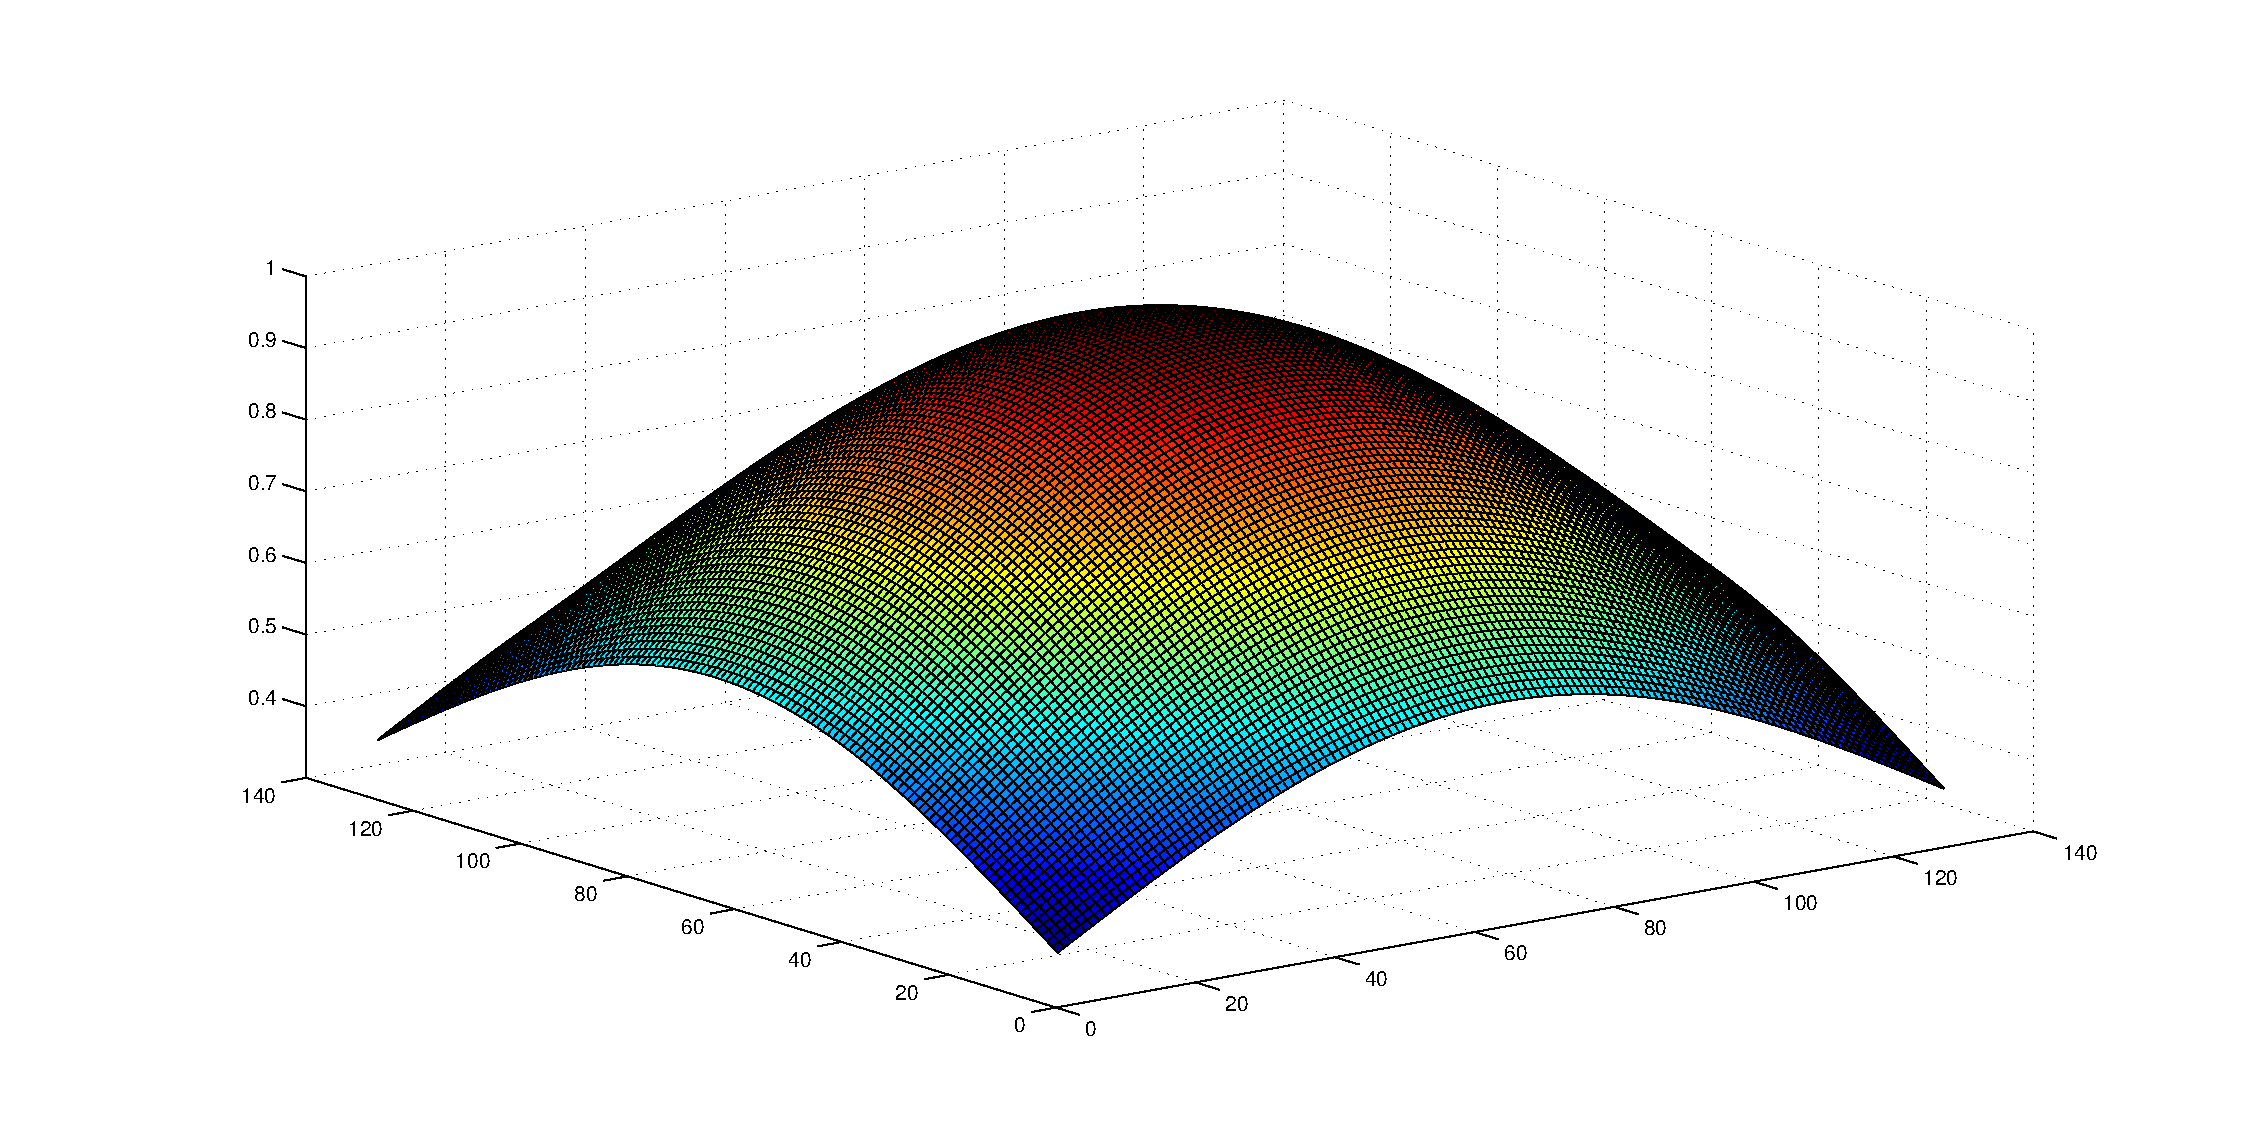
\includegraphics[scale=0.2]{./images/Q14/t01_icc.eps}
      	\caption{Impulse response of the continuous $g(x,y;\ t)$ for $t=0.1$.}
      	\label{fig:Q14_t01_icc}
    \end{figure}
  \end{minipage}
\end{minipage}
\\

The covariance matrices in this case are:\\

\begin{minipage}{\linewidth}
  \begin{minipage}{0.4\linewidth}
\[
var_D =
\begin{bmatrix}
    0.0133  & 0		 	\\
    0       & 0.0133 	\\
\end{bmatrix}
\]
  \end{minipage}
  \hspace{0.05\linewidth}
  \begin{minipage}{0.4\linewidth}
\[
var_C =
\begin{bmatrix}
    9.8124  & 0		 	\\
    0       & 9.8124 	\\
\end{bmatrix}
\]
  \end{minipage}
\end{minipage}

As we can see the variances appear to be approximately ten times less and ten times more than in the ideal case.

\begin{minipage}{\linewidth}
  \begin{minipage}{0.4\linewidth}
    \begin{figure}[H]
    	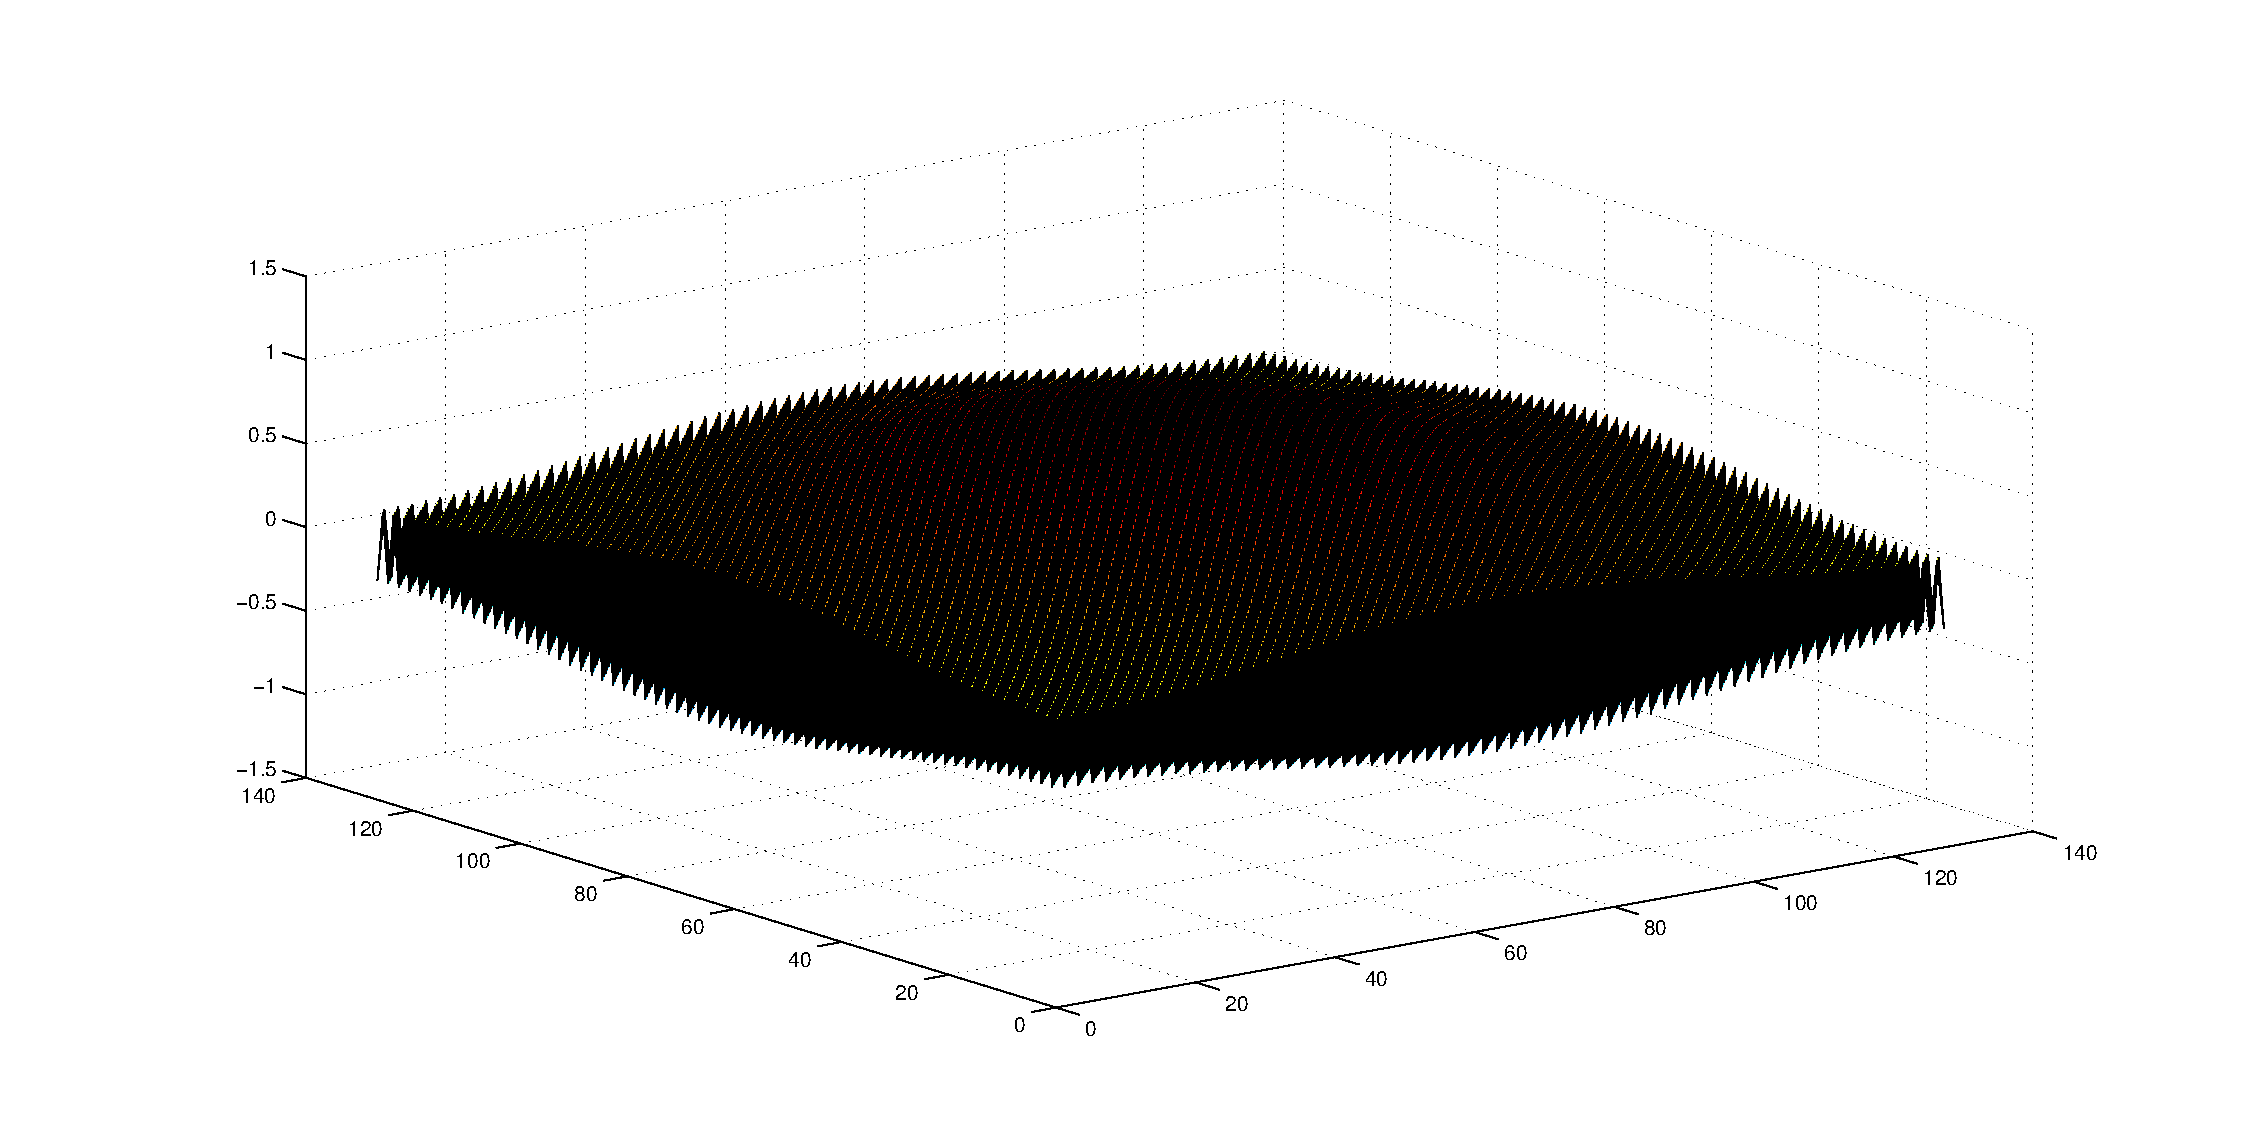
\includegraphics[scale=0.2]{./images/Q14/t03.eps}
      	\caption{Impulse response of the discretized $g(m,n;\ t)$ for $t=0.3$.}
      	\label{fig:Q14_t03}
    \end{figure}
  \end{minipage}
  \hspace{0.05\linewidth}
  \begin{minipage}{0.4\linewidth}
    \begin{figure}[H]
        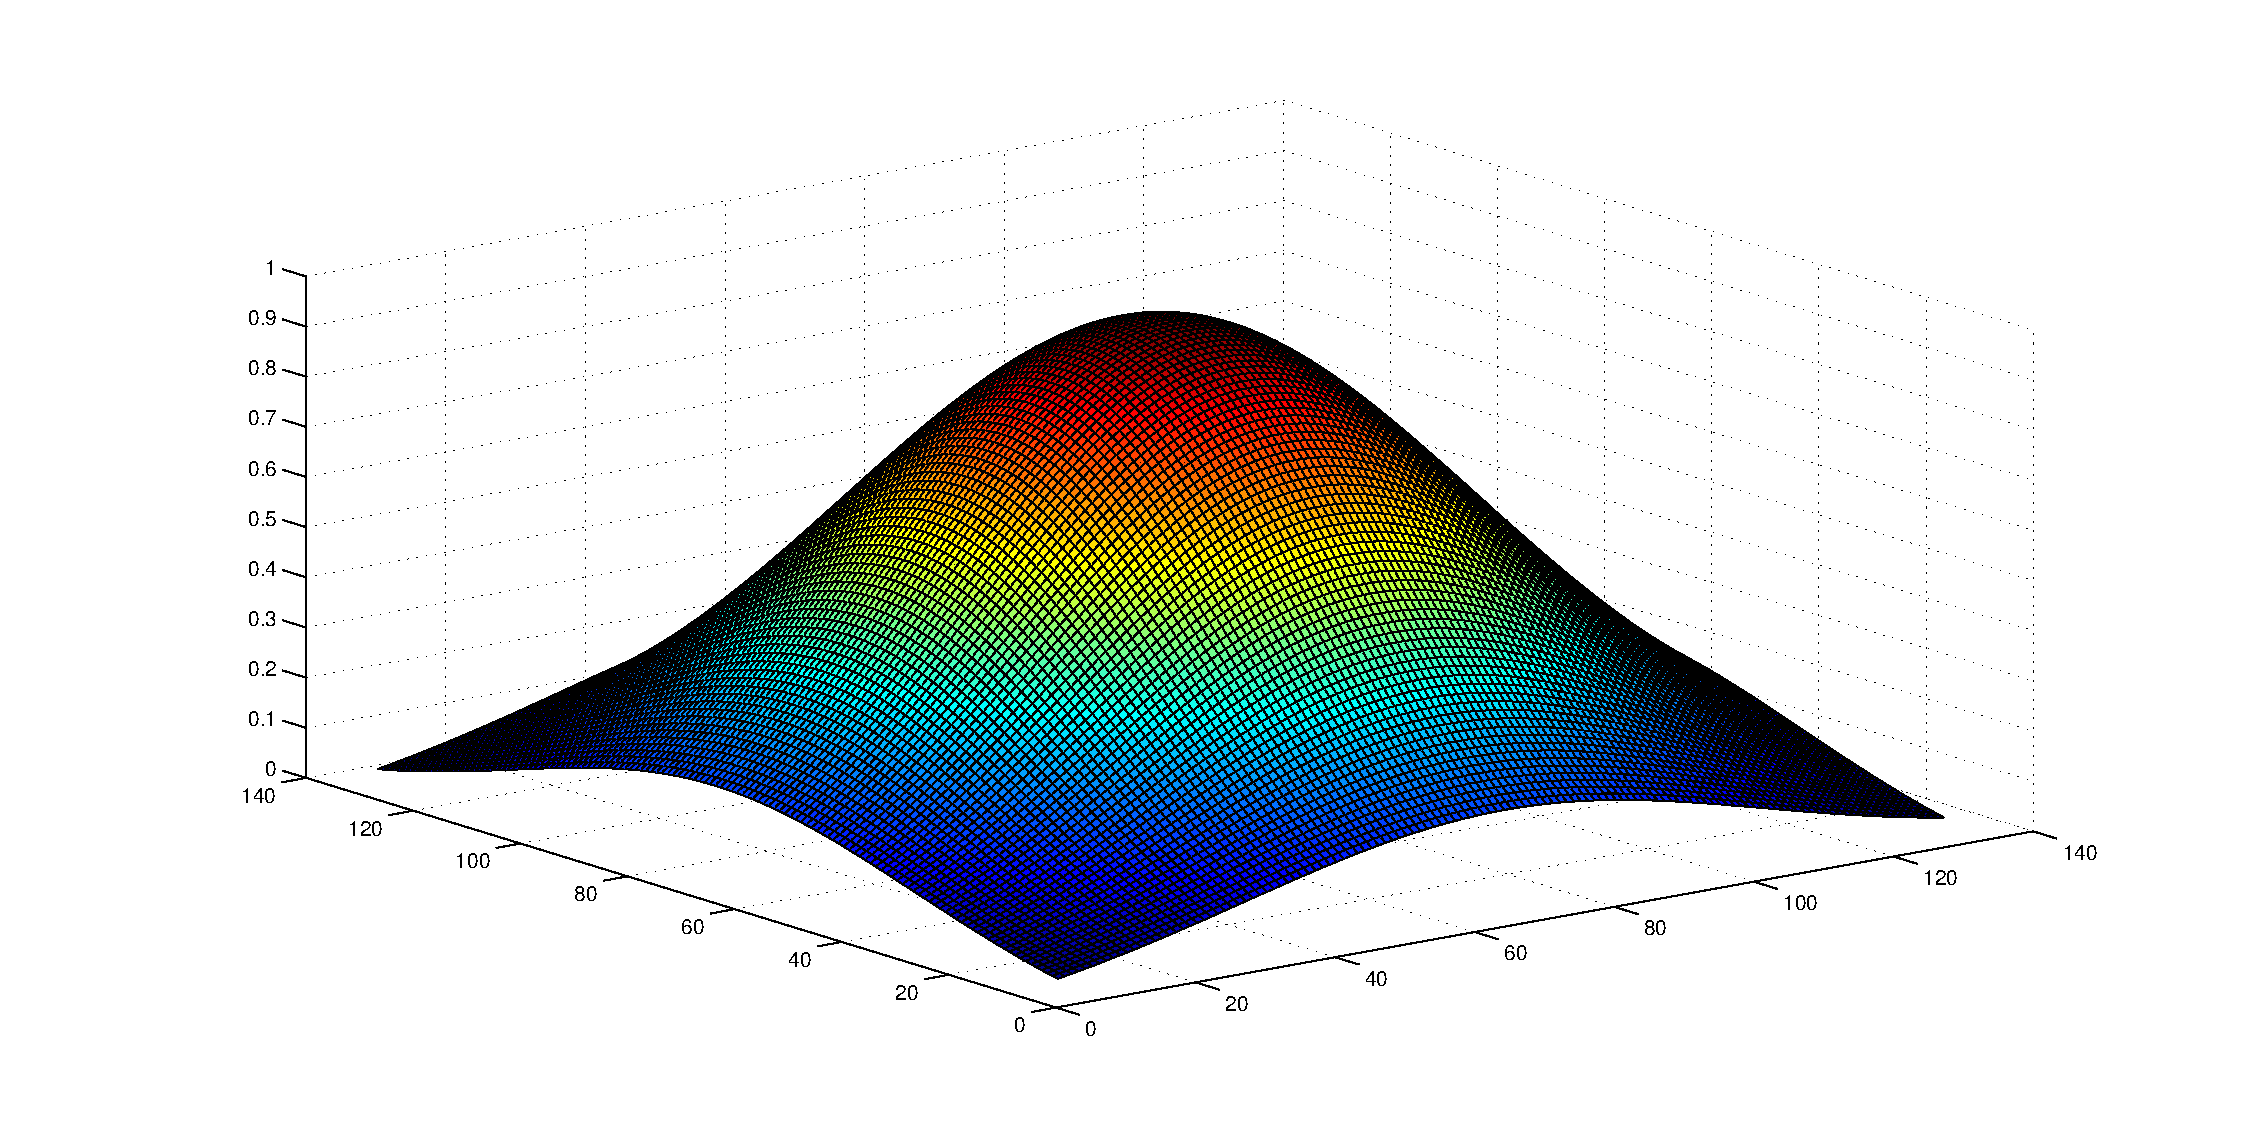
\includegraphics[scale=0.2]{./images/Q14/t03_icc.eps}
      	\caption{Impulse response of the continuous $g(x,y;\ t)$ for $t=0.3$.}
      	\label{fig:Q14_t03_icc}
    \end{figure}
  \end{minipage}
\end{minipage}
\\

The covariance matrices in this case are:\\

\begin{minipage}{\linewidth}
  \begin{minipage}{0.4\linewidth}
\[
var_D =
\begin{bmatrix}
    0.2811  & 0		 	\\
    0       & 0.2811 	\\
\end{bmatrix}
\]
  \end{minipage}
  \hspace{0.05\linewidth}
  \begin{minipage}{0.4\linewidth}
\[
var_C =
\begin{bmatrix}
    11.0845  & 0		 	\\
    0        & 11.0845124 	\\
\end{bmatrix}
\]
  \end{minipage}
\end{minipage}


\begin{minipage}{\linewidth}
  \begin{minipage}{0.4\linewidth}
    \begin{figure}[H]
    	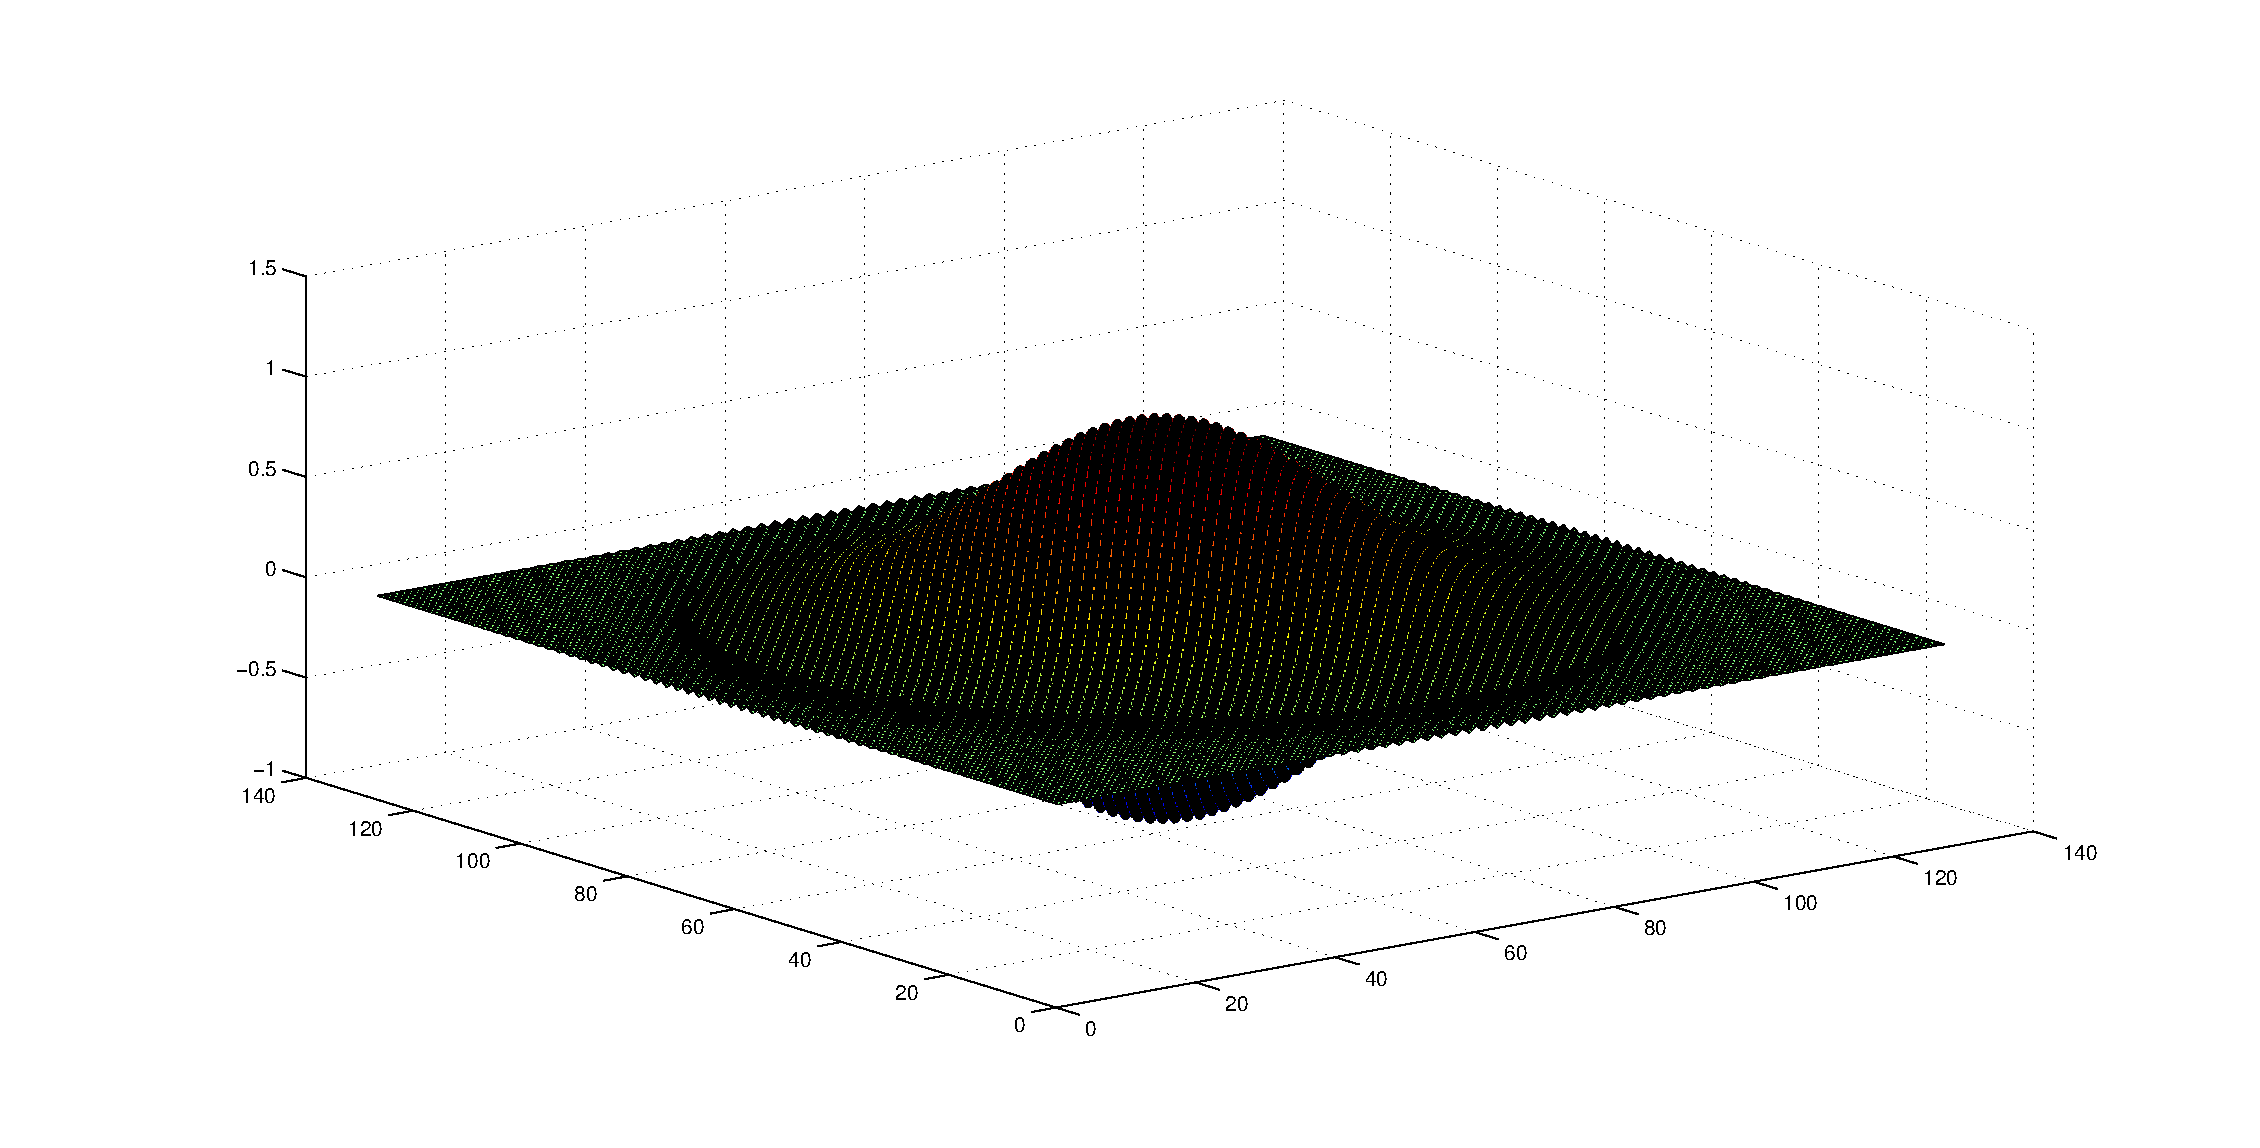
\includegraphics[scale=0.2]{./images/Q14/t1.eps}
      	\caption{Impulse response of the discretized $g(m,n;\ t)$ for $t=1$.}
      	\label{fig:Q14_t1}
    \end{figure}
  \end{minipage}
  \hspace{0.05\linewidth}
  \begin{minipage}{0.4\linewidth}
    \begin{figure}[H]
        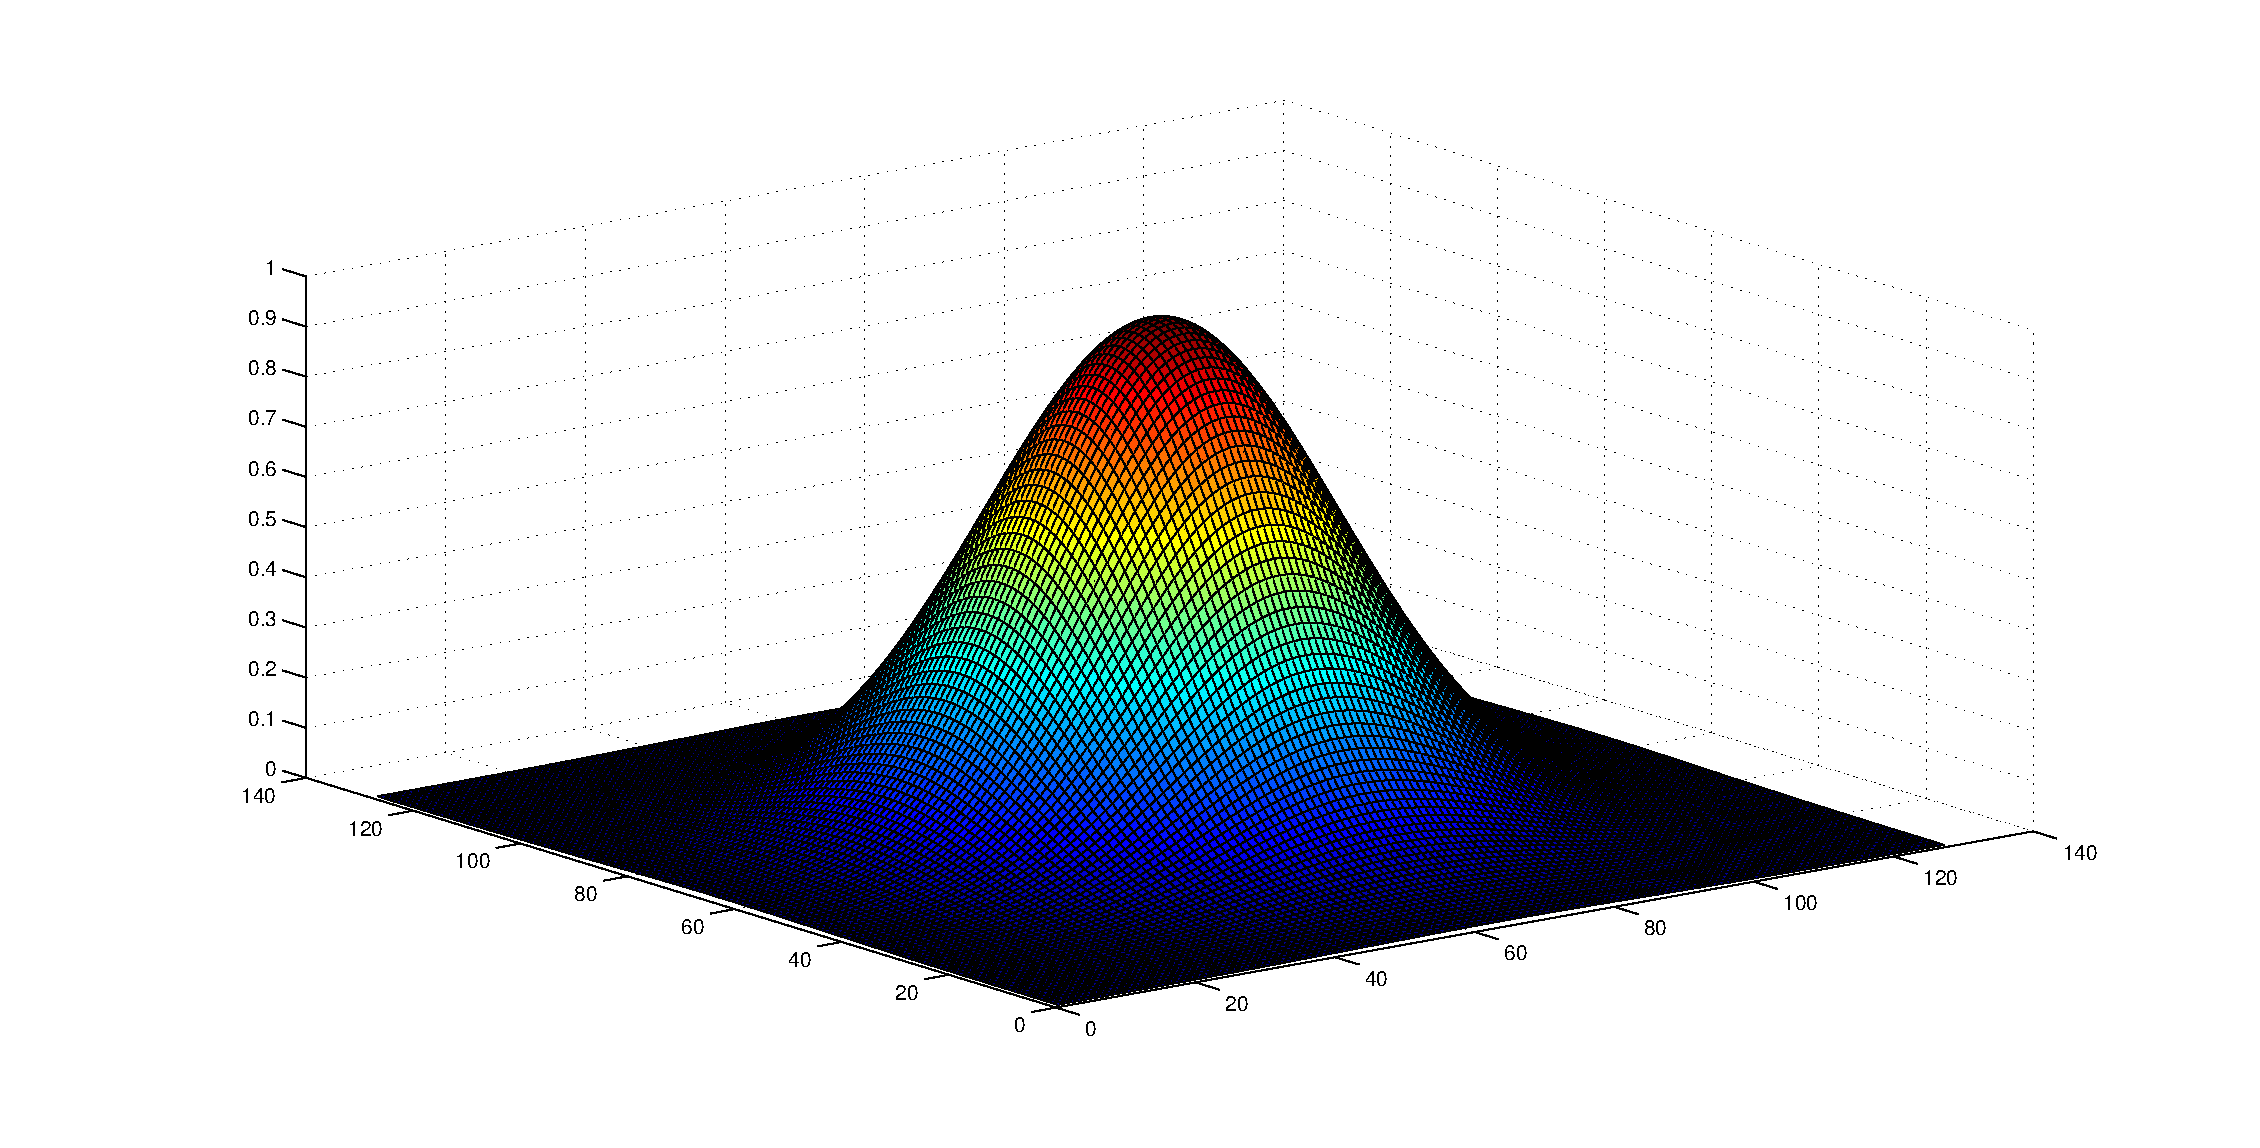
\includegraphics[scale=0.2]{./images/Q14/t1_icc.eps}
      	\caption{Impulse response of the continuous $g(x,y;\ t)$ for $t=1$.}
      	\label{fig:Q14_t1_icc}
    \end{figure}
  \end{minipage}
\end{minipage}
\\

The covariance matrices in this case are:\\

\begin{minipage}{\linewidth}
  \begin{minipage}{0.4\linewidth}
\[
var_D =
\begin{bmatrix}
    1.0  & 0		 	\\
    0       & 1.0 	 	\\
\end{bmatrix}
\]
  \end{minipage}
  \hspace{0.05\linewidth}
  \begin{minipage}{0.4\linewidth}
\[
var_C =
\begin{bmatrix}
	2.1898  & 0		 	\\
    0       & 2.1898 	\\
\end{bmatrix}
\]
  \end{minipage}
\end{minipage}

\begin{minipage}{\linewidth}
  \begin{minipage}{0.4\linewidth}
    \begin{figure}[H]
    	\includegraphics[scale=0.2]{./images/Q14/t10.eps}
      	\caption{Impulse response of the discretized $g(m,n;\ t)$ for $t=10$.}
      	\label{fig:Q14_t10}
    \end{figure}
  \end{minipage}
  \hspace{0.05\linewidth}
  \begin{minipage}{0.4\linewidth}
    \begin{figure}[H]
        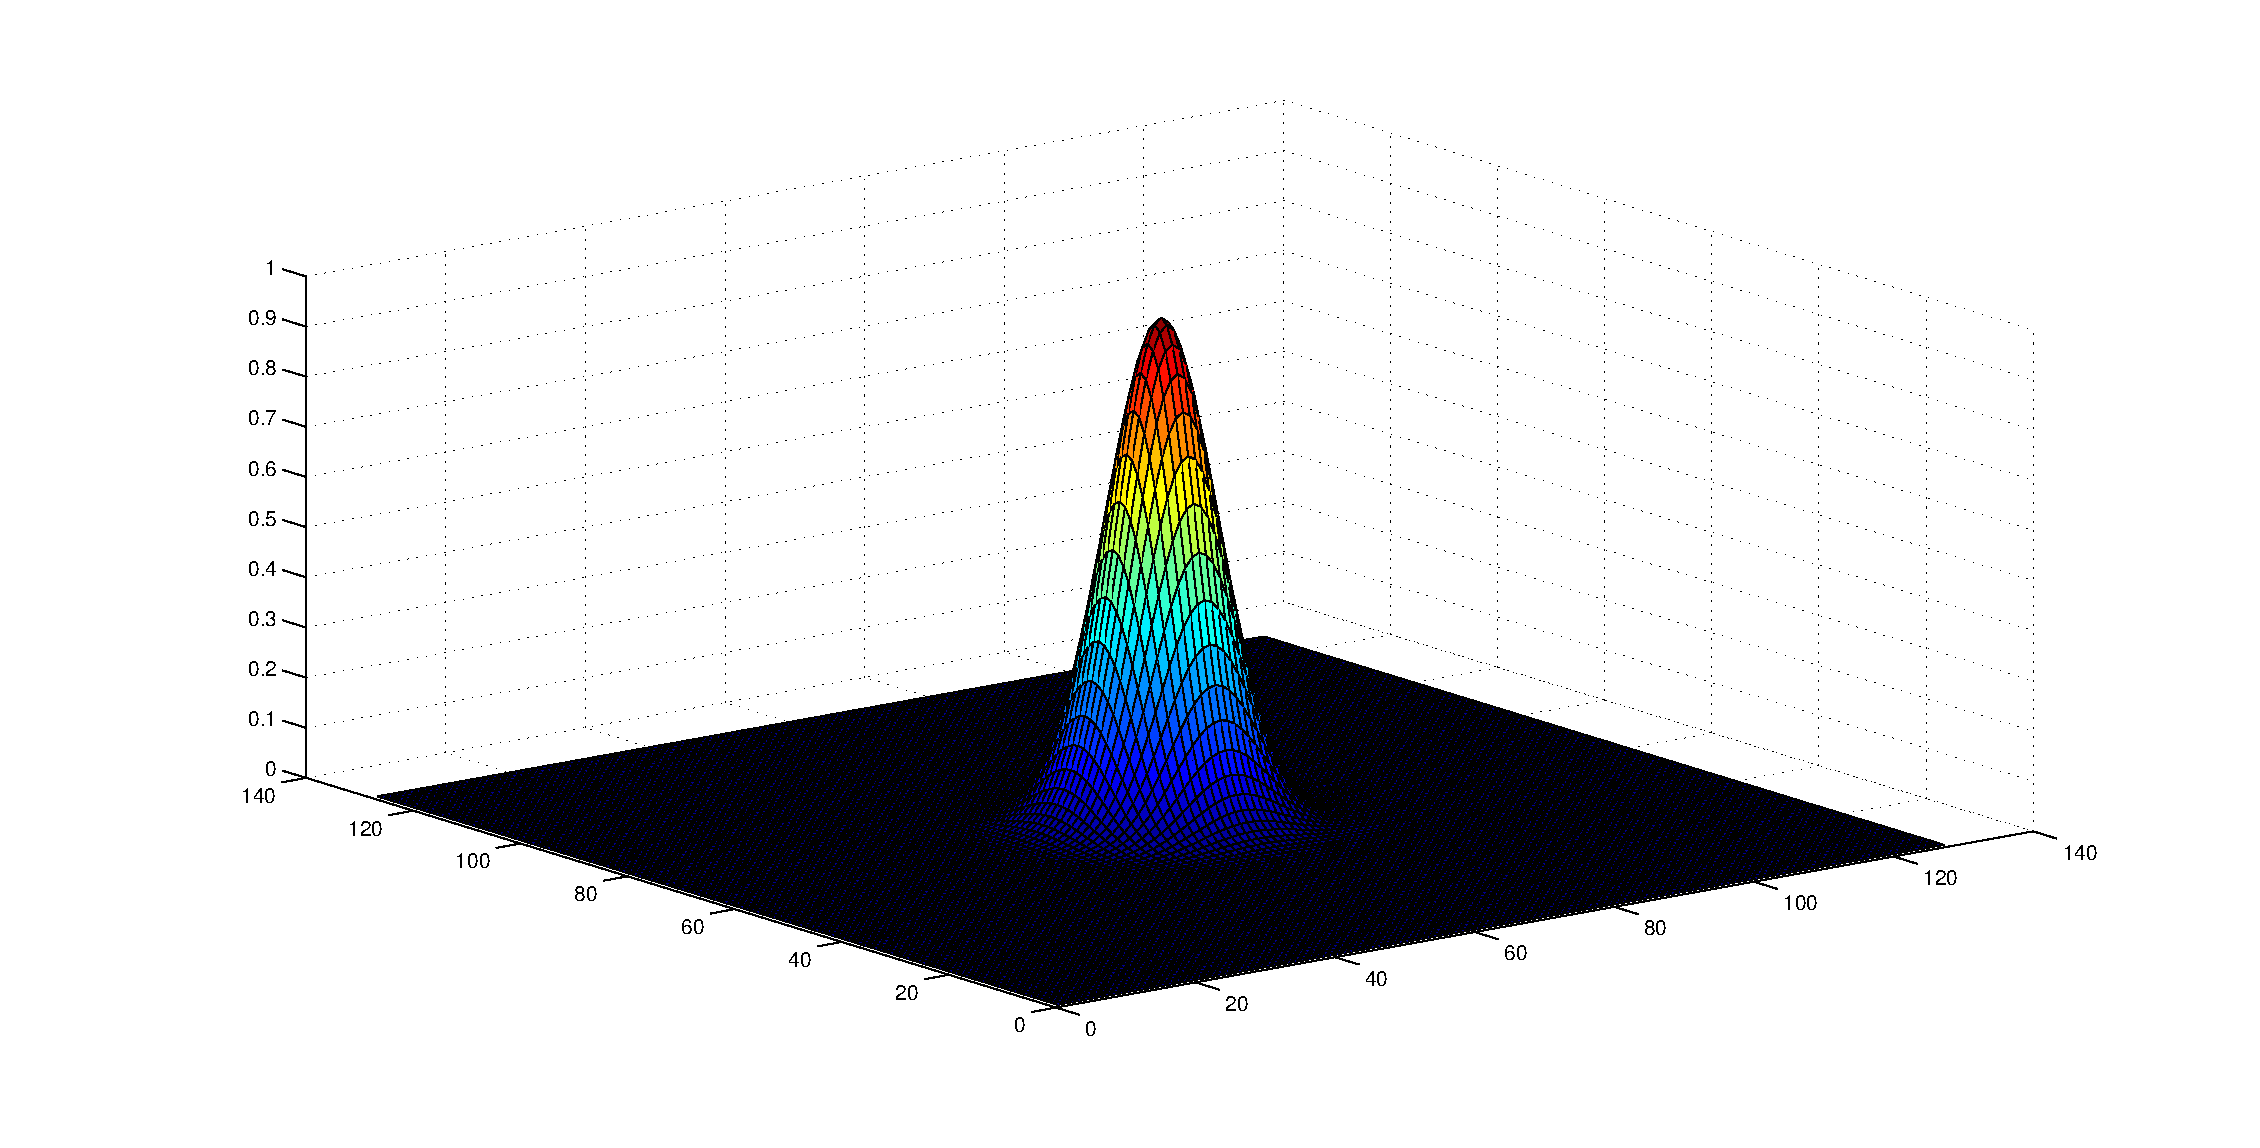
\includegraphics[scale=0.2]{./images/Q14/t10_icc.eps}
      	\caption{Impulse response of the continuous $g(x,y;\ t)$ for $t=10$.}
      	\label{fig:Q14_t10_icc}
    \end{figure}
  \end{minipage}
\end{minipage}
\\

The covariance matrices in this case are:\\

\begin{minipage}{\linewidth}
  \begin{minipage}{0.4\linewidth}
\[
var_D =
\begin{bmatrix}
    10.0  	& 0		 	\\
    0       & 10.0 	\\
\end{bmatrix}
\]
  \end{minipage}
  \hspace{0.05\linewidth}
  \begin{minipage}{0.4\linewidth}
\[
var_C =
\begin{bmatrix}
    10.0	 & 0		 	\\
    0        & 10.0 	\\
\end{bmatrix}
\]
  \end{minipage}
\end{minipage}


\begin{minipage}{\linewidth}
  \begin{minipage}{0.4\linewidth}
    \begin{figure}[H]
    	\includegraphics[scale=0.2]{./images/Q14/t100.eps}
      	\caption{Impulse response of the discretized $g(m,n;\ t)$ for $t=100$.}
      	\label{fig:Q14_t100}
    \end{figure}
  \end{minipage}
  \hspace{0.05\linewidth}
  \begin{minipage}{0.4\linewidth}
    \begin{figure}[H]
        \includegraphics[scale=0.2]{./images/Q14/t100_icc.eps}
      	\caption{Impulse response of the continuous $g(x,y;\ t)$ for $t=100$.}
      	\label{fig:Q14_t100_icc}
    \end{figure}
  \end{minipage}
\end{minipage}
\\

The covariance matrices in this case are:\\

\begin{minipage}{\linewidth}
  \begin{minipage}{0.4\linewidth}
\[
var_D =
\begin{bmatrix}
    100.0   & 0		 	\\
    0       & 100.0 	\\
\end{bmatrix}
\]
  \end{minipage}
  \hspace{0.05\linewidth}
  \begin{minipage}{0.4\linewidth}
\[
var_C =
\begin{bmatrix}
    100.0  & 0		 	\\
    0      & 100.0 	\\
\end{bmatrix}
\]
  \end{minipage}
\end{minipage}
\\


In the case of the discrete Gaussian kernel, its impulse response for various values of $t$ is shown in figures \ref{fig:Q14_t01_disc} - \ref{fig:Q14_t100_disc}.


\begin{minipage}{\linewidth}
  \begin{minipage}{0.4\linewidth}
    \begin{figure}[H]
    	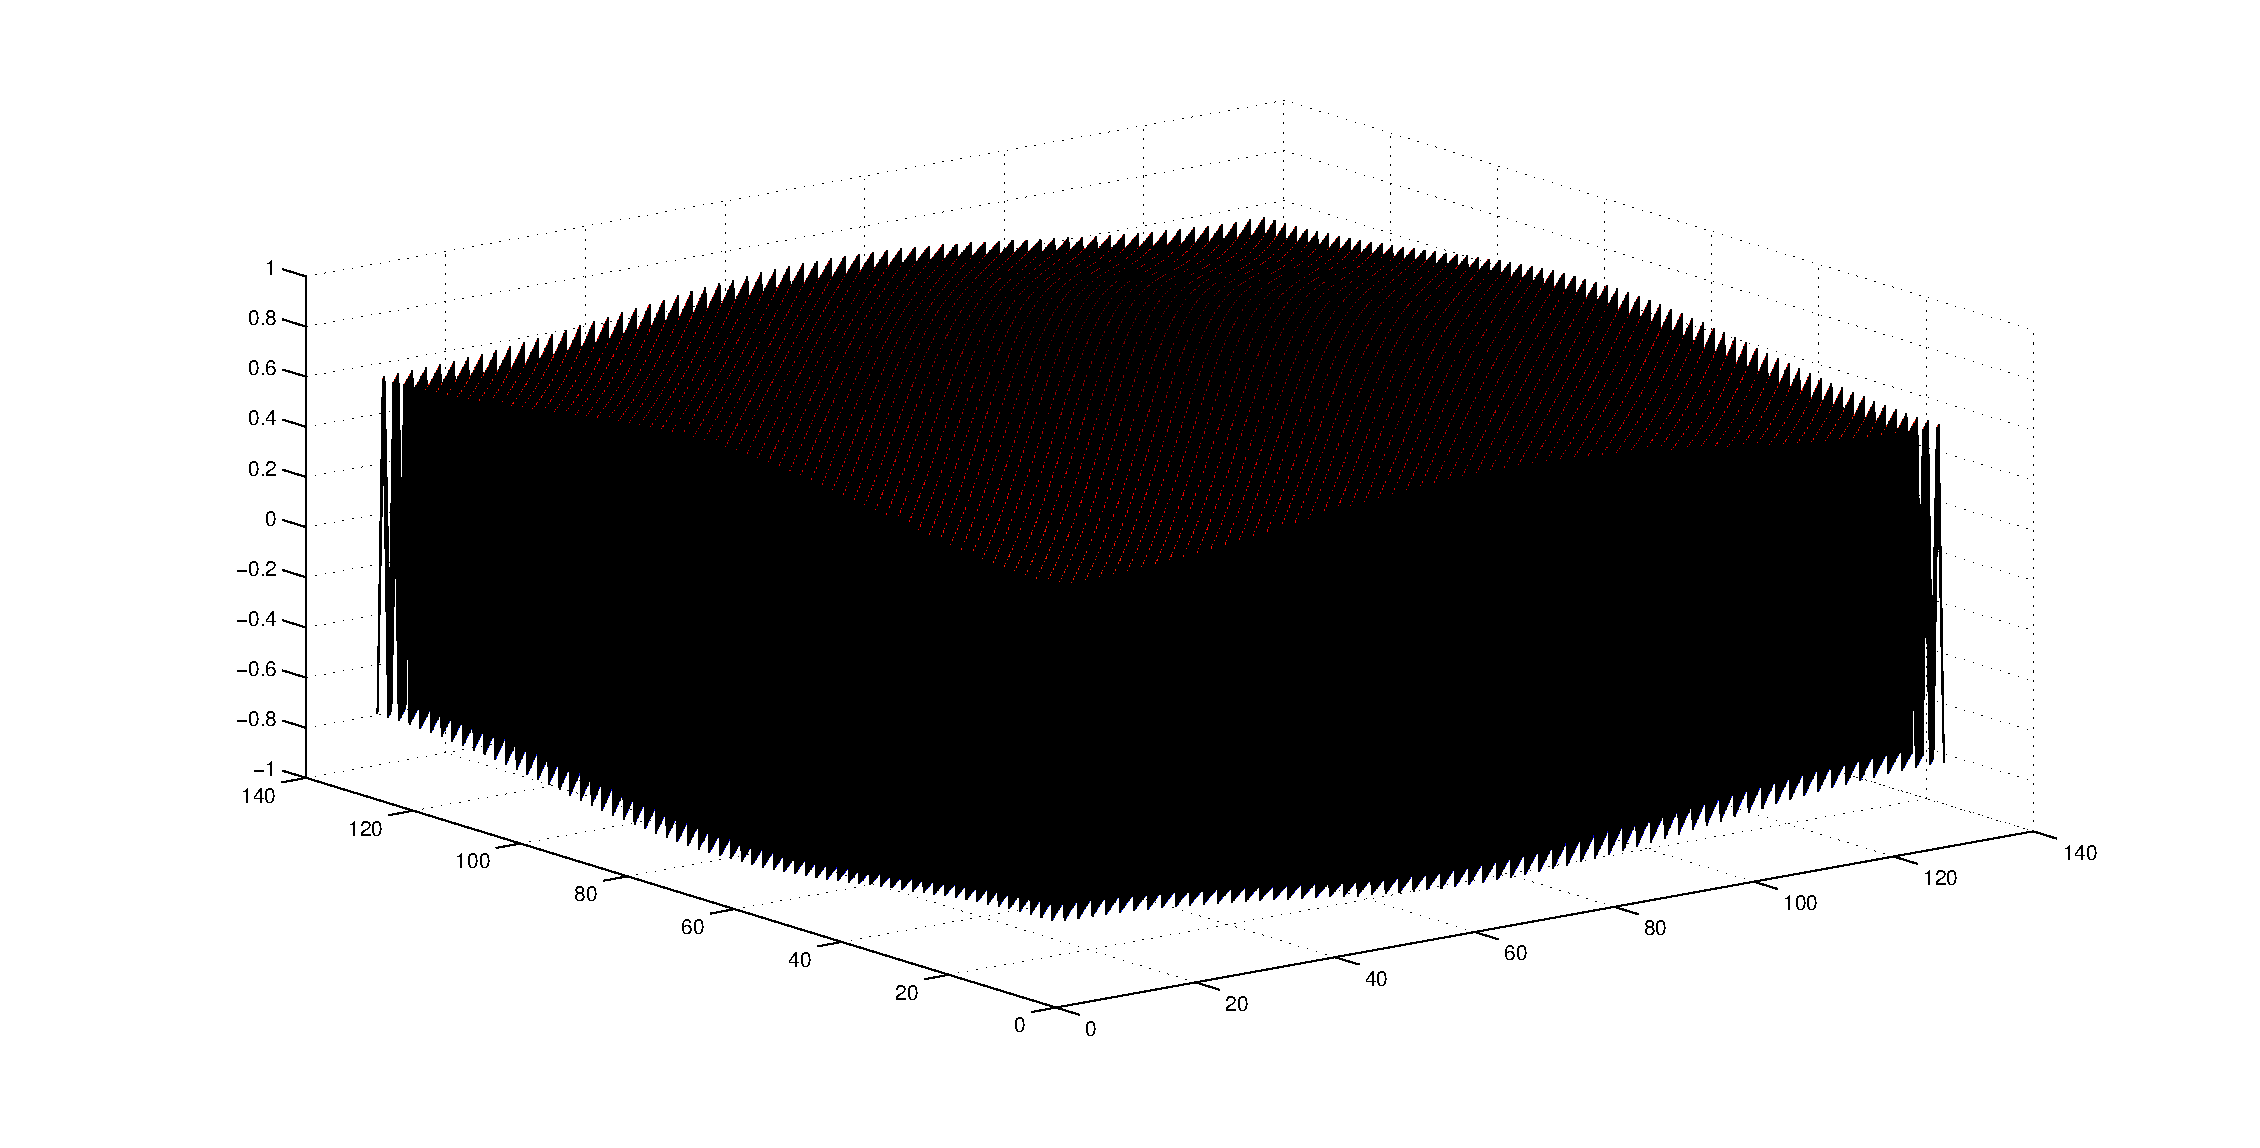
\includegraphics[scale=0.2]{./images/Q14/t01_disc.eps}
      	\caption{Impulse response of the discretized $g(m,n;\ t)$ for $t=0.1$, using the \texttt{discgaussfft} method.}
      	\label{fig:Q14_t01_disc}
    \end{figure}
  \end{minipage}
  \hspace{0.05\linewidth}
  \begin{minipage}{0.4\linewidth}
    \begin{figure}[H]
        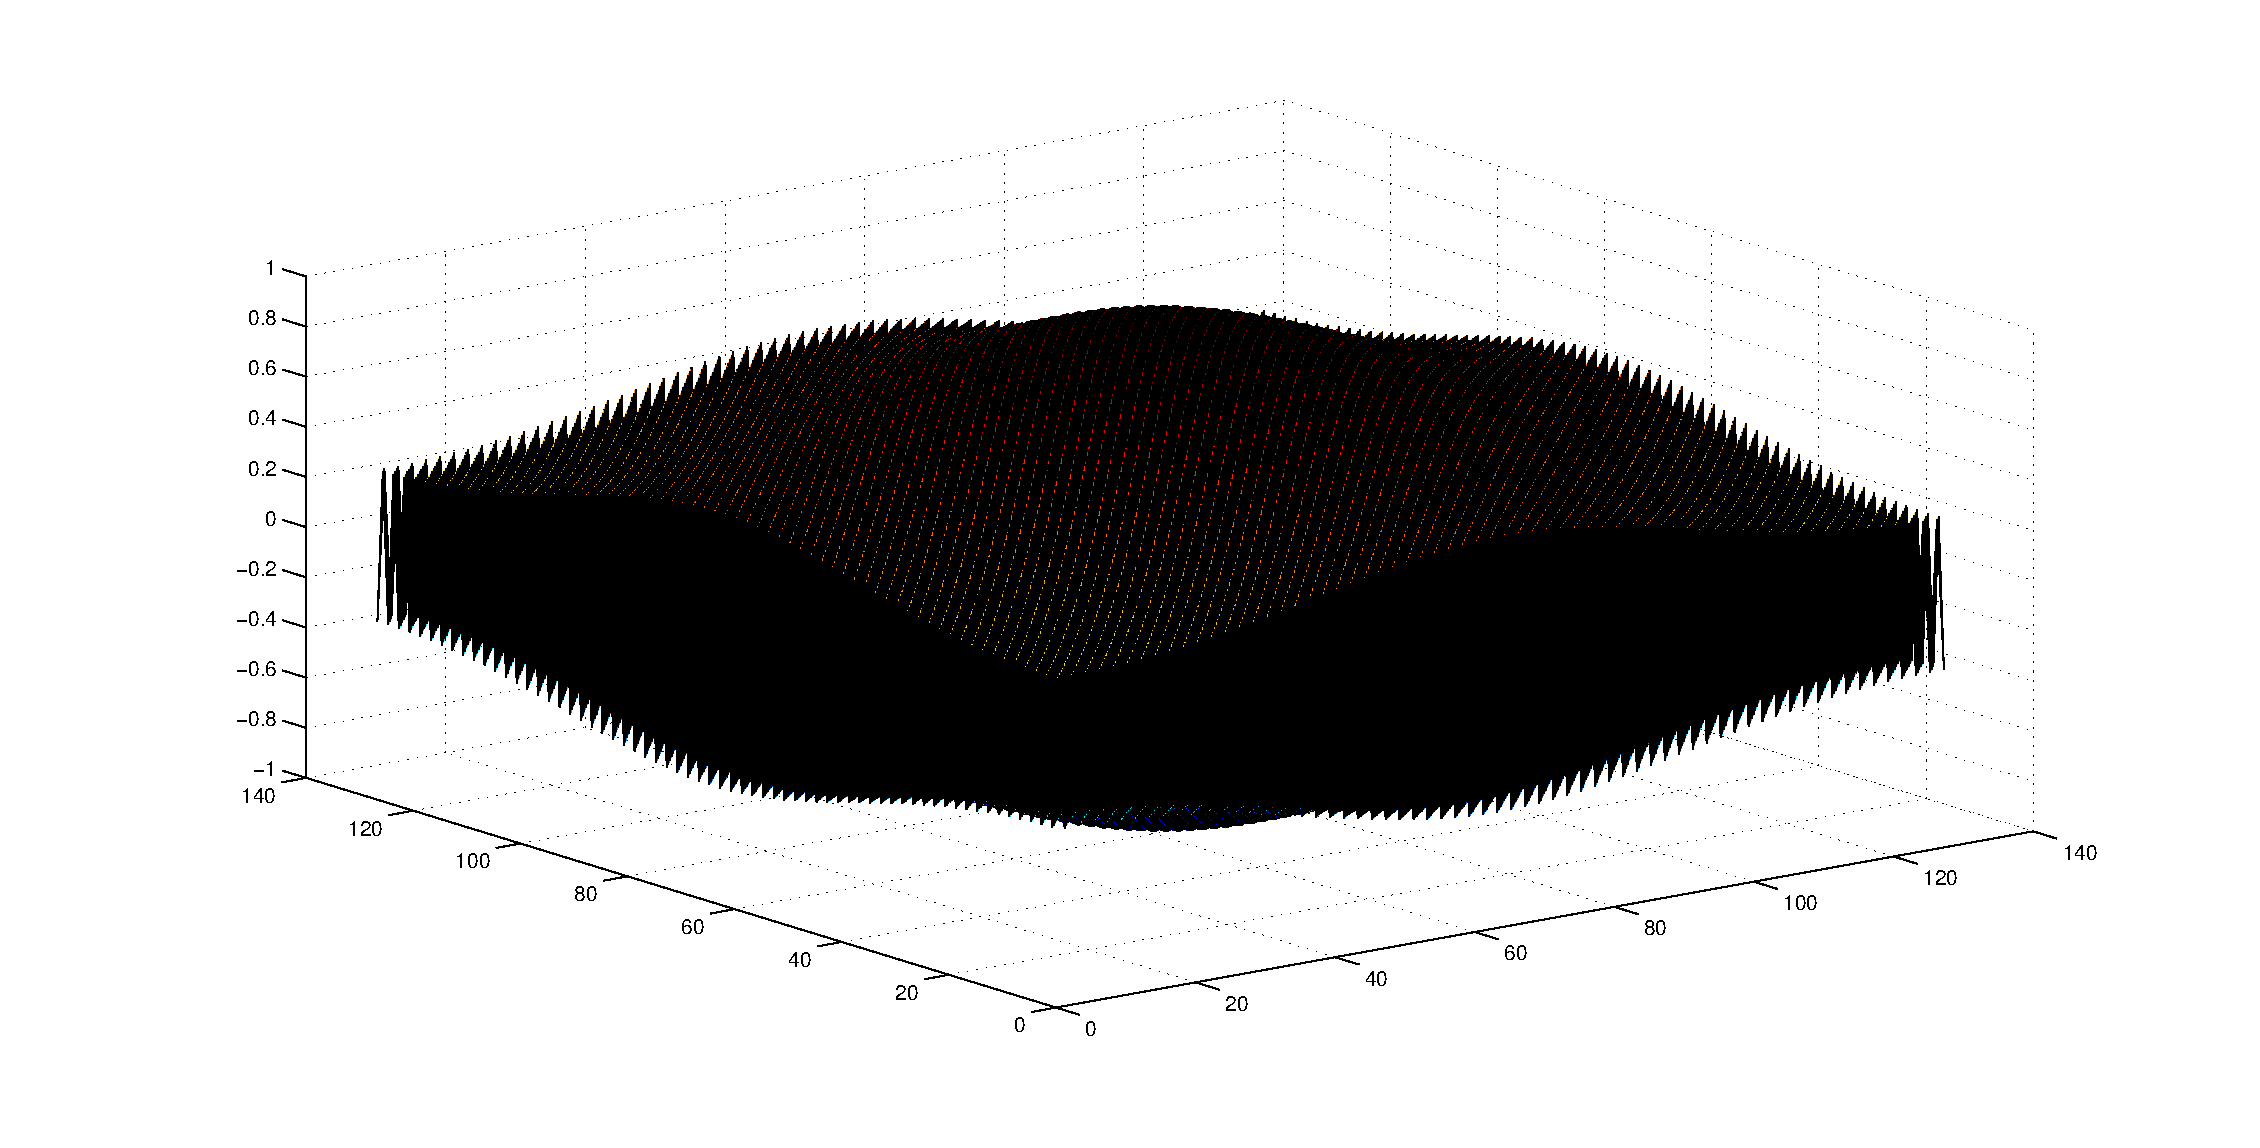
\includegraphics[scale=0.2]{./images/Q14/t03_disc.eps}
      	\caption{Impulse response of the discretized $g(m,n;\ t)$ for $t=0.3$, using the \texttt{discgaussfft} method.}
      	\label{fig:Q14_t03_disc}
    \end{figure}
  \end{minipage}
\end{minipage}


\begin{minipage}{\linewidth}
  \begin{minipage}{0.4\linewidth}
    \begin{figure}[H]
    	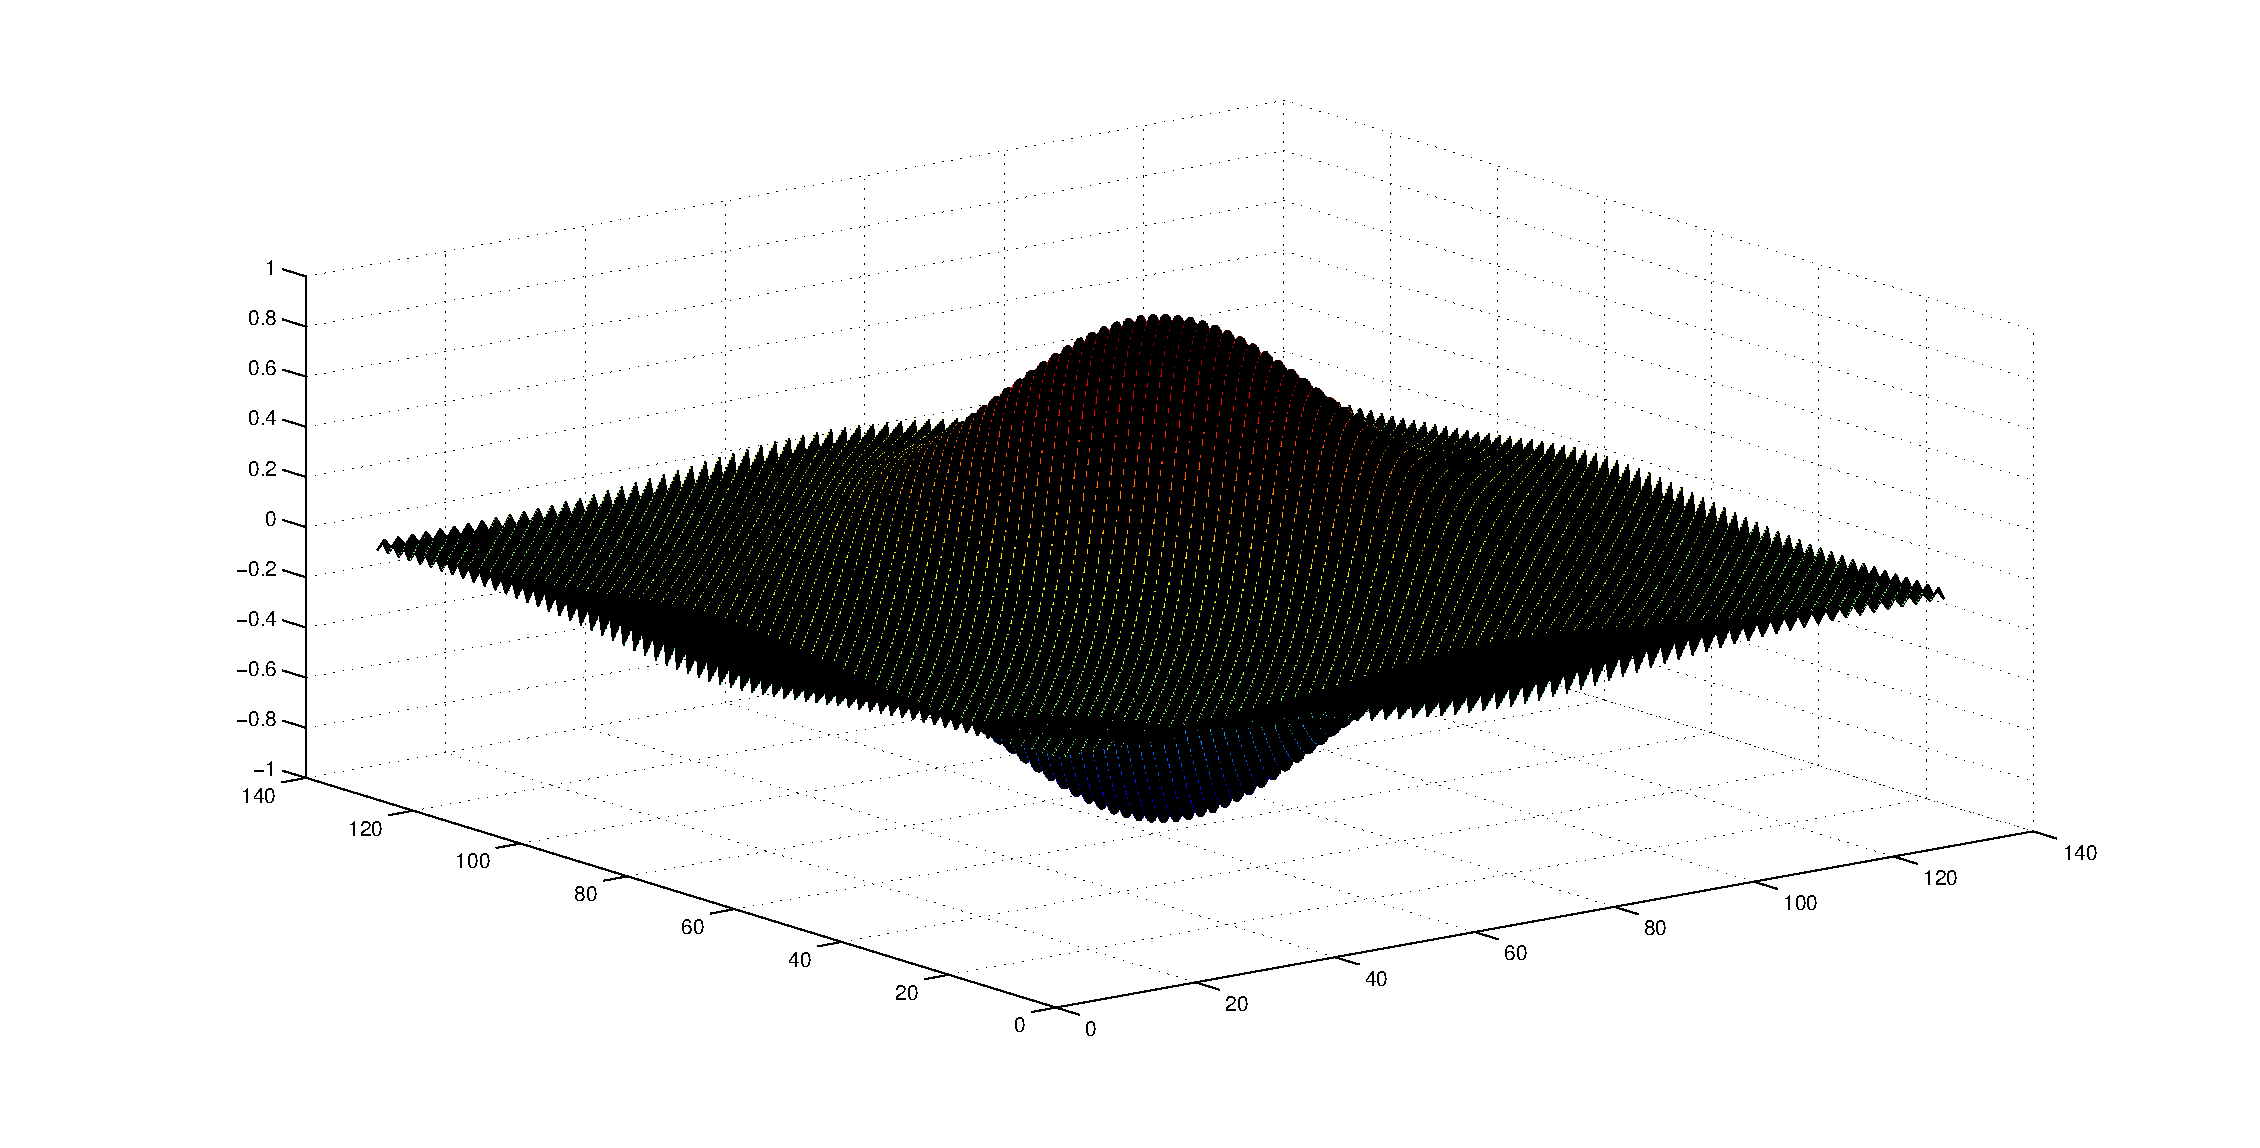
\includegraphics[scale=0.2]{./images/Q14/t1_disc.eps}
      	\caption{Impulse response of the discretized $g(m,n;\ t)$ for $t=1$, using the \texttt{discgaussfft} method.}
      	\label{fig:Q14_t1_disc}
    \end{figure}
  \end{minipage}
  \hspace{0.05\linewidth}
  \begin{minipage}{0.4\linewidth}
    \begin{figure}[H]
        \includegraphics[scale=0.2]{./images/Q14/t10_disc.eps}
      	\caption{Impulse response of the discretized $g(m,n;\ t)$ for $t=10$, using the \texttt{discgaussfft} method.}
      	\label{fig:Q14_t10_disc}
    \end{figure}
  \end{minipage}
\end{minipage}

\begin{minipage}{\linewidth}
  \begin{minipage}{0.4\linewidth}
    \begin{figure}[H]
    	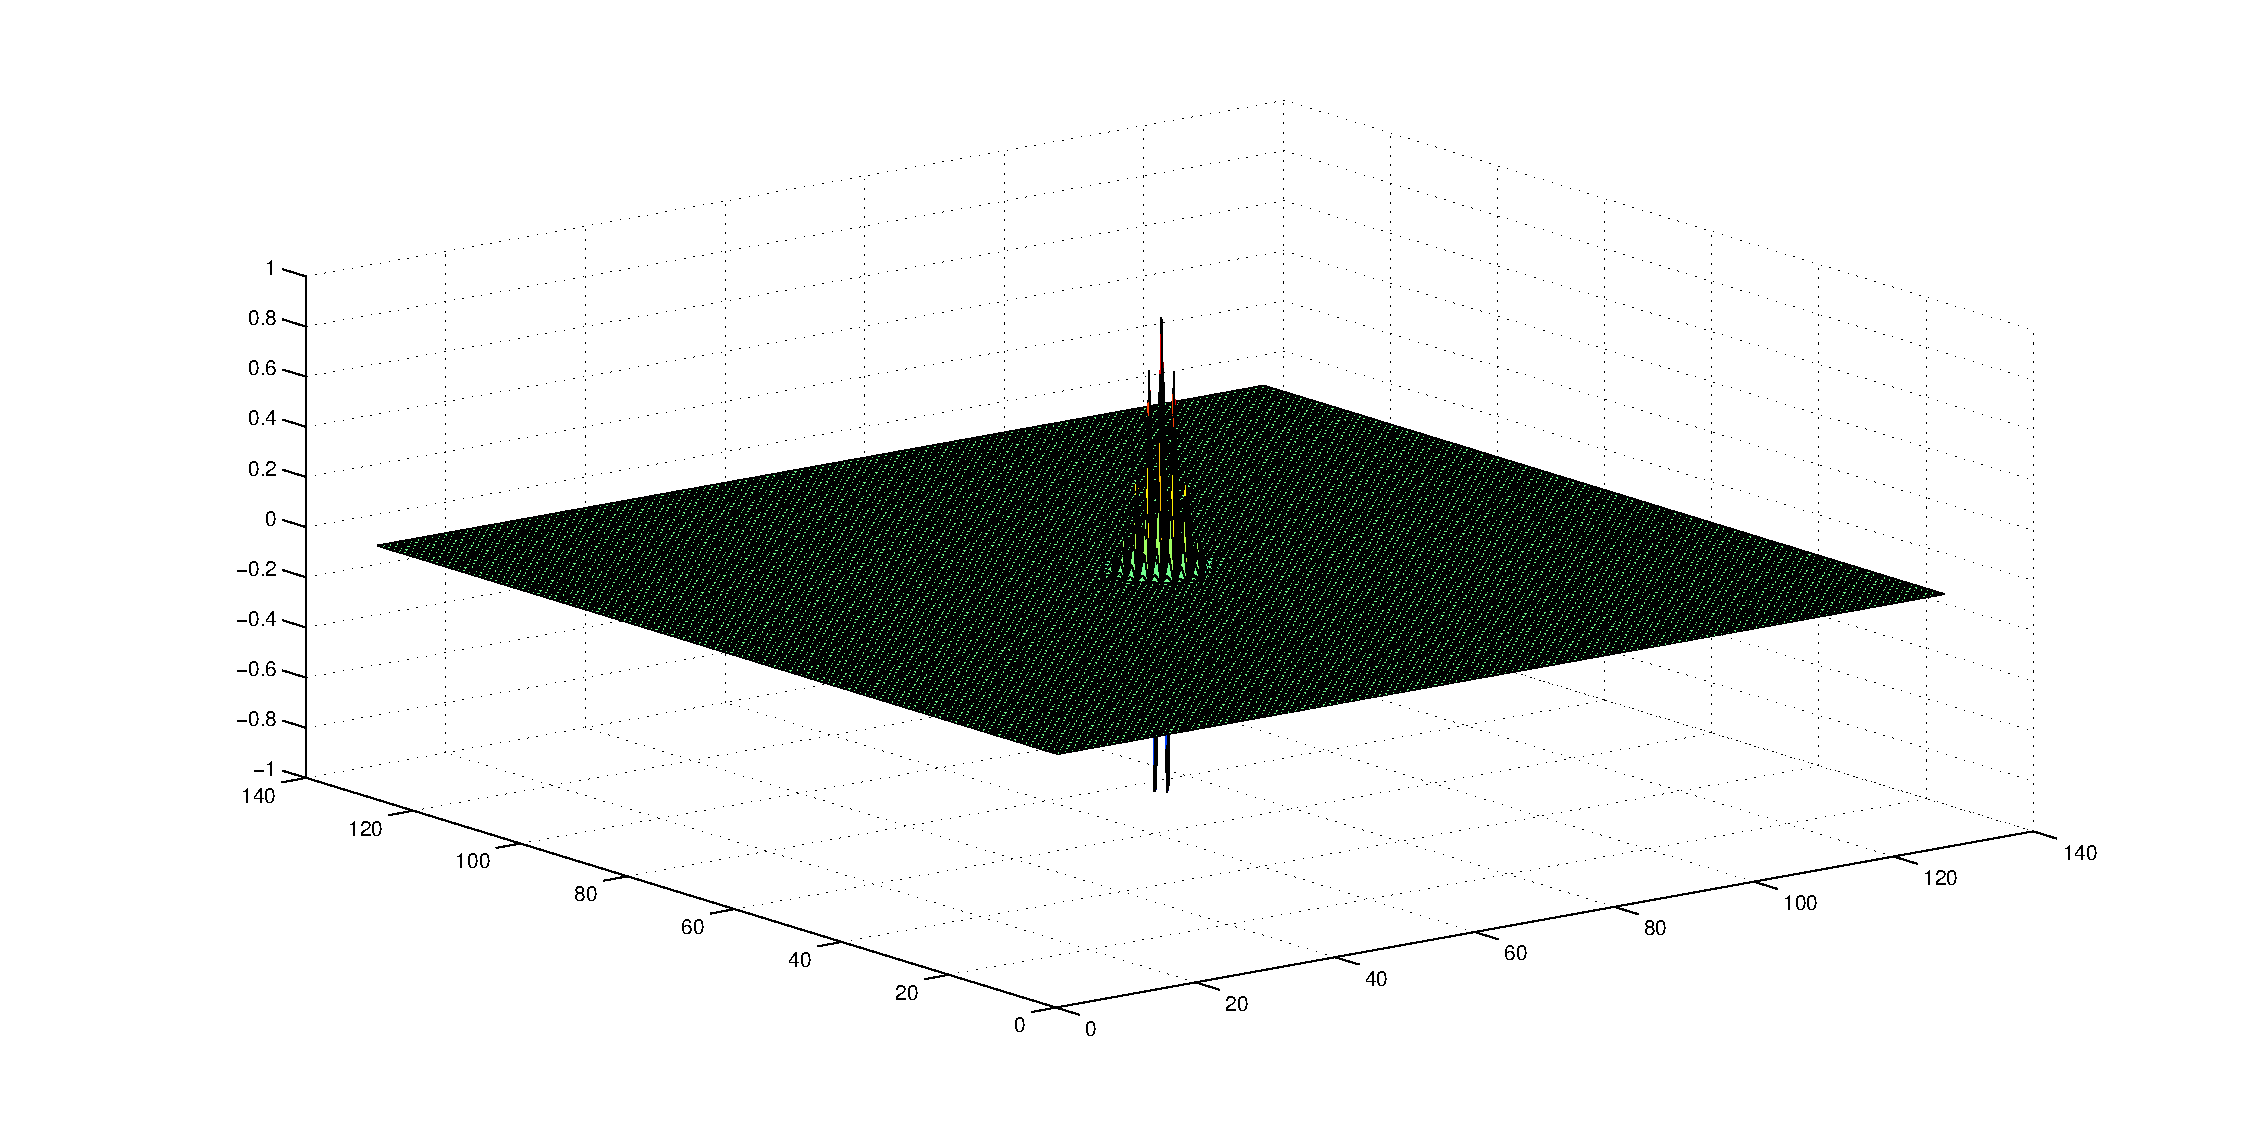
\includegraphics[scale=0.2]{./images/Q14/t100_disc.eps}
      	\caption{Impulse response of the discretized $g(m,n;\ t)$ for $t=100$, using the \texttt{discgaussfft} method.}
      	\label{fig:Q14_t100_disc}
    \end{figure}
  \end{minipage}
  \hspace{0.05\linewidth}
  \begin{minipage}{0.5\linewidth}
As for their variance, it is indeed \[
var = t \cdot
\begin{bmatrix}
    1  & 0		 	\\
    0      & 1 	\\
\end{bmatrix}
\]

\end{minipage}
\end{minipage}
\\

\subsection{Question 15}

As seen in figures \ref{fig:Q14_t01}, \ref{fig:Q14_t03}, \ref{fig:Q14_t1}, \ref{fig:Q14_t10} and \ref{fig:Q14_t100}, the first two surfaces do not represent
a Gaussian distribution. In fact, only if the values for $t$ are more than $\pi / 4$ they will be Gaussians. Only then can we compare their variances
to the ones of the discretized Gaussian kernel.

\subsection{Question 16}

Figures \ref{fig:Q16_phone_original}, \ref{fig:Q16_few_original} and \ref{fig:Q16_nallo_original} show the original \texttt{phonecalc128}, \texttt{few128} and
\texttt{nallo128} images. Figures \ref{fig:Q16_phone_1} - \ref{fig:Q16_nallo_256} illustrate the effect of the application of a Gaussian filter for various
values of $t$.

\begin{minipage}{\linewidth}
  \begin{minipage}{0.25\linewidth}
    \begin{figure}[H]
      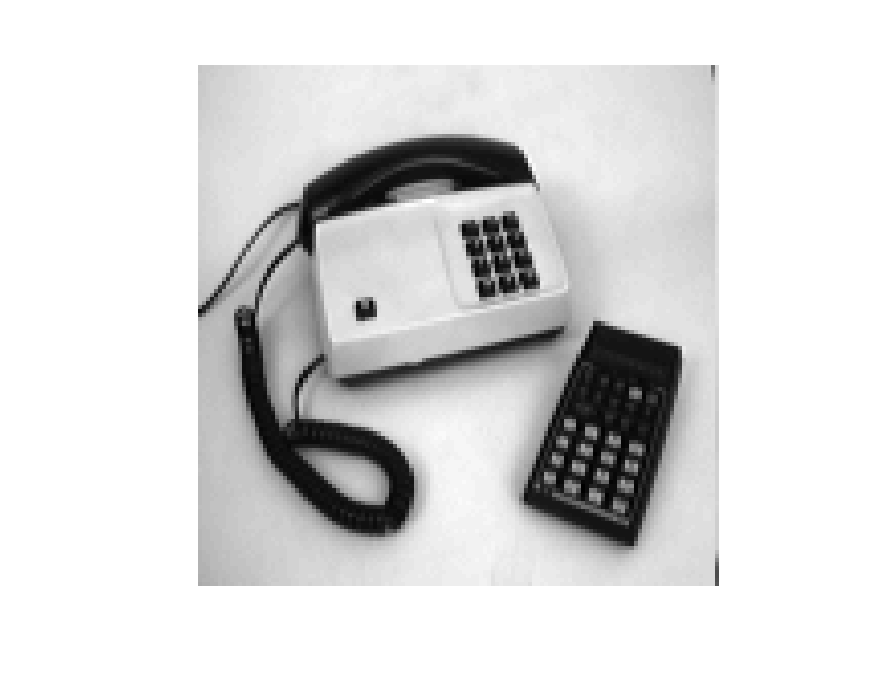
\includegraphics[scale=0.5]{./images/Q16/phone_original.eps}
      \caption{The origin \texttt{phonecalc128} image.}
      \label{fig:Q16_phone_original}
    \end{figure}
  \end{minipage}
  \hspace{0.05\linewidth}
  \begin{minipage}{0.25\linewidth}
    \begin{figure}[H]
      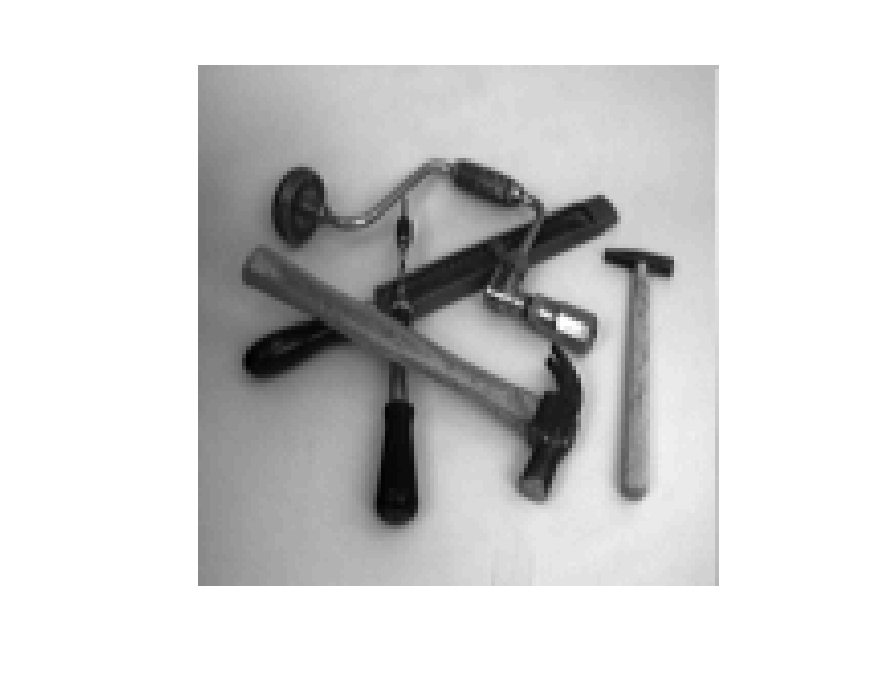
\includegraphics[scale=0.5]{./images/Q16/few_original.eps}
      \caption{The origin \texttt{few128} image.}
      \label{fig:Q16_few_original}
    \end{figure}
  \end{minipage}
    \hspace{0.05\linewidth}
  \begin{minipage}{0.25\linewidth}
    \begin{figure}[H]
      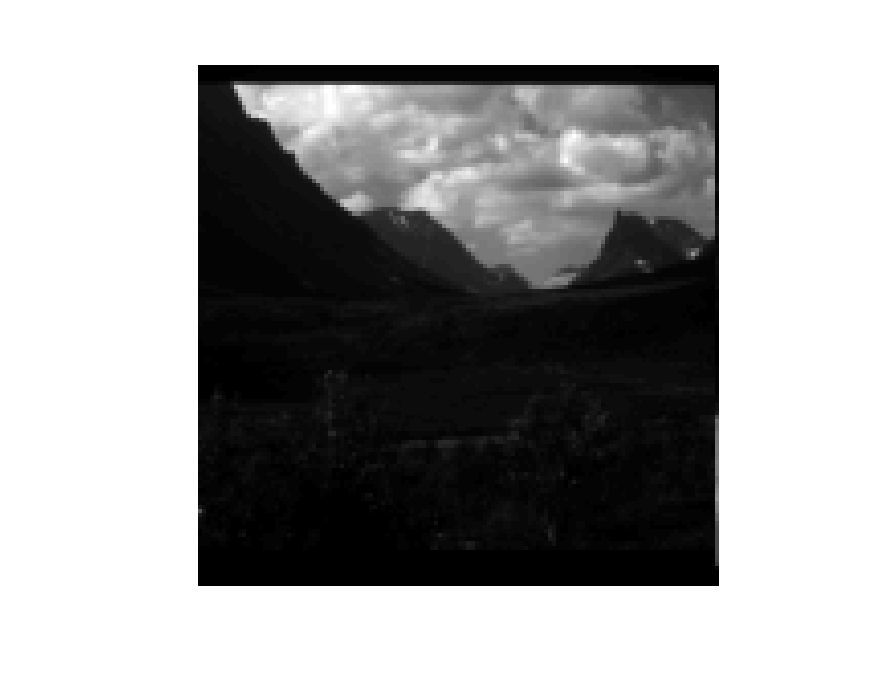
\includegraphics[scale=0.5]{./images/Q16/nallo_original.eps}
      \caption{The origin \texttt{nallo128} image.}
      \label{fig:Q16_nallo_original}
    \end{figure}
  \end{minipage}
\end{minipage}
\\

\begin{minipage}{\linewidth}
  \begin{minipage}{0.25\linewidth}
    \begin{figure}[H]
      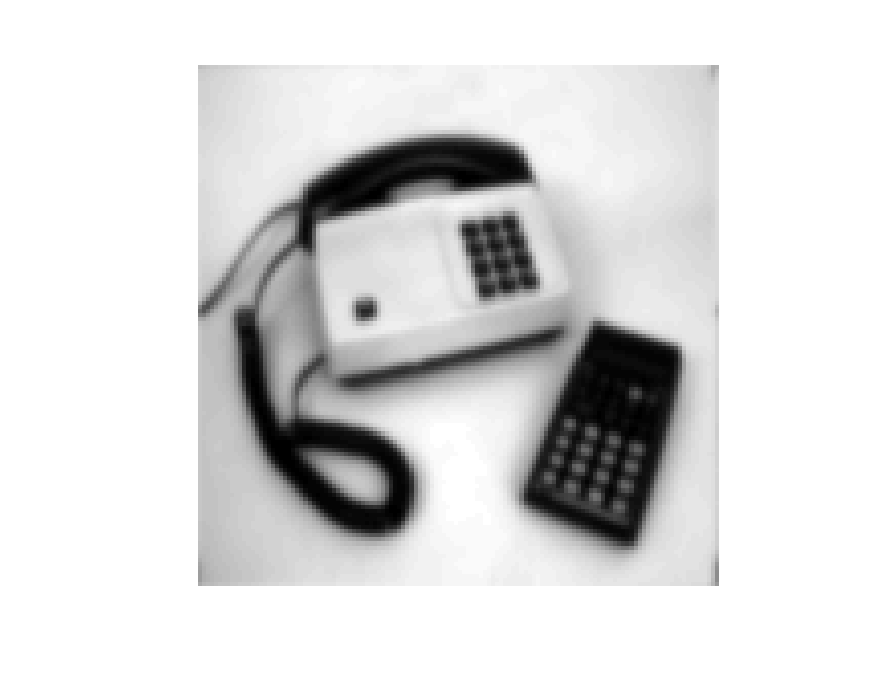
\includegraphics[scale=0.5]{./images/Q16/phone_1.eps}
      \caption{The result of the application of a gaussian function with $t=1$ to image \texttt{phonecalc128}.}
      \label{fig:Q16_phone_1}
    \end{figure}
  \end{minipage}
  \hspace{0.05\linewidth}
  \begin{minipage}{0.25\linewidth}
    \begin{figure}[H]
      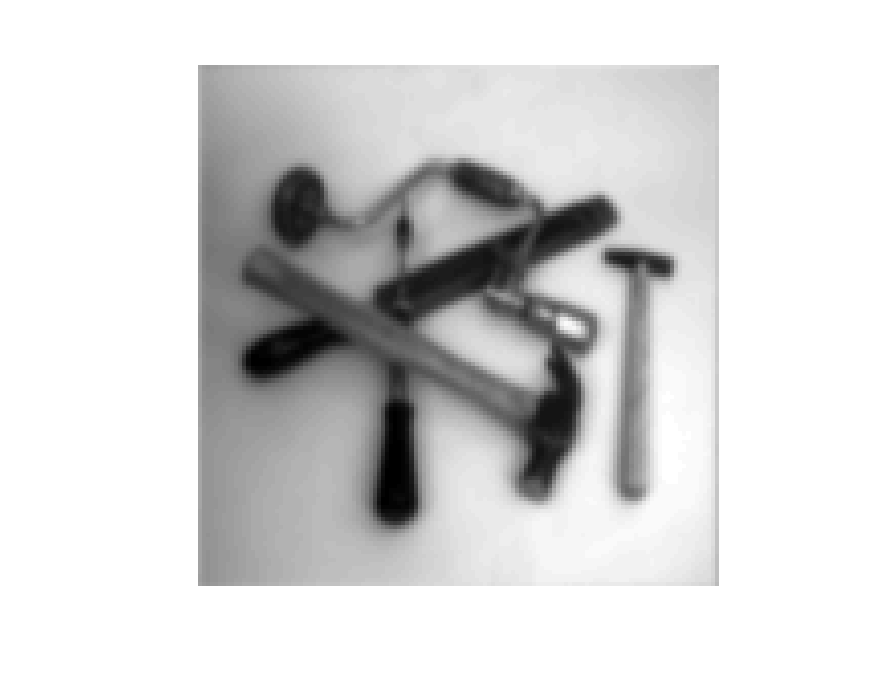
\includegraphics[scale=0.5]{./images/Q16/few_1.eps}
      \caption{The result of the application of a gaussian function with $t=1$ to image \texttt{few128}.}
      \label{fig:Q16_few_1}
    \end{figure}
  \end{minipage}
    \hspace{0.05\linewidth}
  \begin{minipage}{0.25\linewidth}
    \begin{figure}[H]
      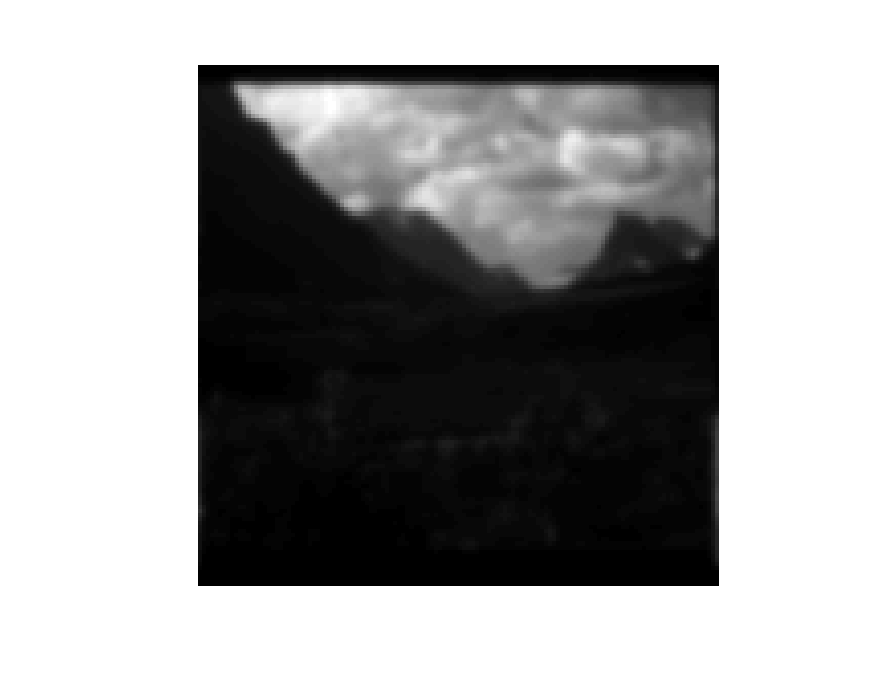
\includegraphics[scale=0.5]{./images/Q16/nallo_1.eps}
      \caption{The result of the application of a gaussian function with $t=1$ to image \texttt{nallo128}.}
      \label{fig:Q16_nallo_1}
    \end{figure}
  \end{minipage}
\end{minipage}
\\


\begin{minipage}{\linewidth}
  \begin{minipage}{0.25\linewidth}
    \begin{figure}[H]
      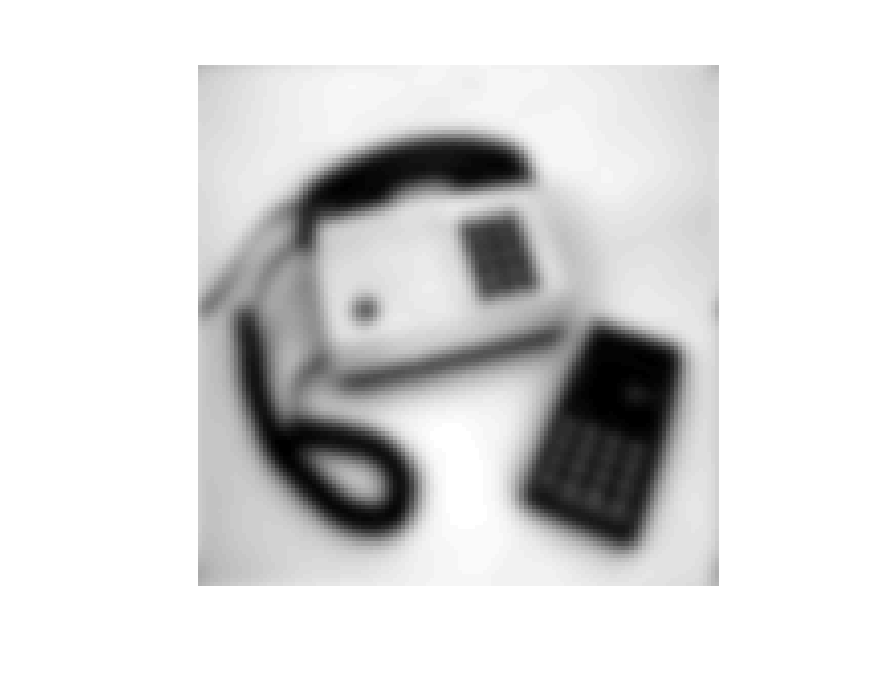
\includegraphics[scale=0.5]{./images/Q16/phone_4.eps}
      \caption{The result of the application of a gaussian function with $t=4$ to image \texttt{phonecalc128}.}
      \label{fig:Q16_phone_4}
    \end{figure}
  \end{minipage}
  \hspace{0.05\linewidth}
  \begin{minipage}{0.25\linewidth}
    \begin{figure}[H]
      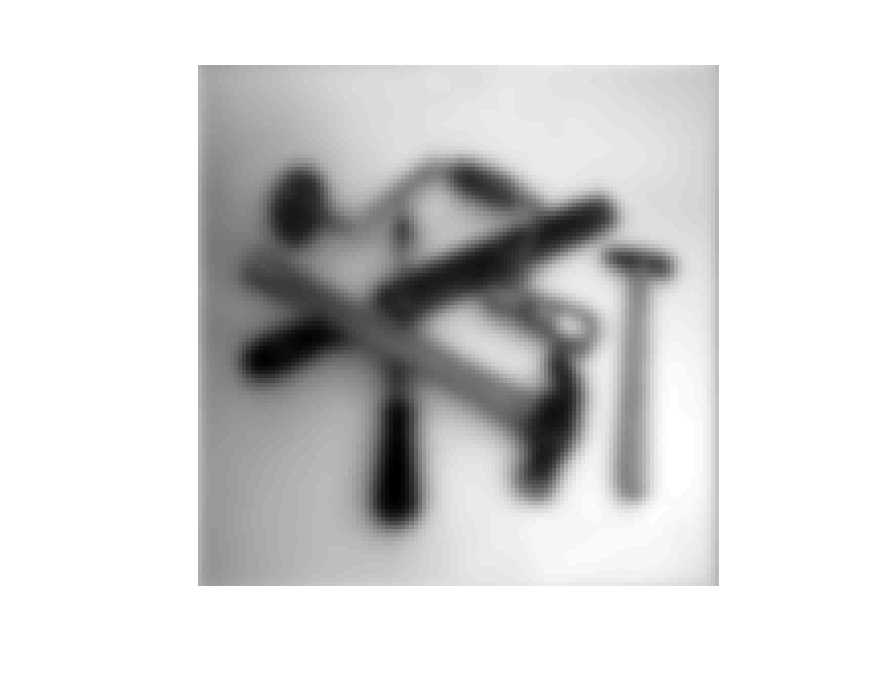
\includegraphics[scale=0.5]{./images/Q16/few_4.eps}
      \caption{The result of the application of a gaussian function with $t=4$ to image \texttt{few128}.}
      \label{fig:Q16_few_4}
    \end{figure}
  \end{minipage}
    \hspace{0.05\linewidth}
  \begin{minipage}{0.25\linewidth}
    \begin{figure}[H]
      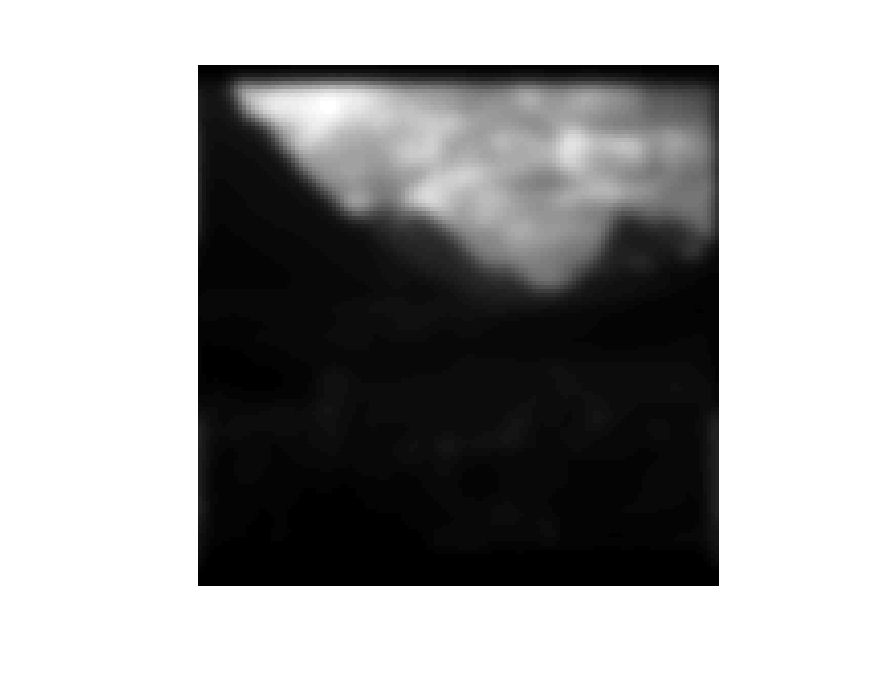
\includegraphics[scale=0.5]{./images/Q16/nallo_4.eps}
      \caption{The result of the application of a gaussian function with $t=4$ to image \texttt{nallo128}.}
      \label{fig:Q16_nallo_4}
    \end{figure}
  \end{minipage}
\end{minipage}
\\


\begin{minipage}{\linewidth}
  \begin{minipage}{0.25\linewidth}
    \begin{figure}[H]
      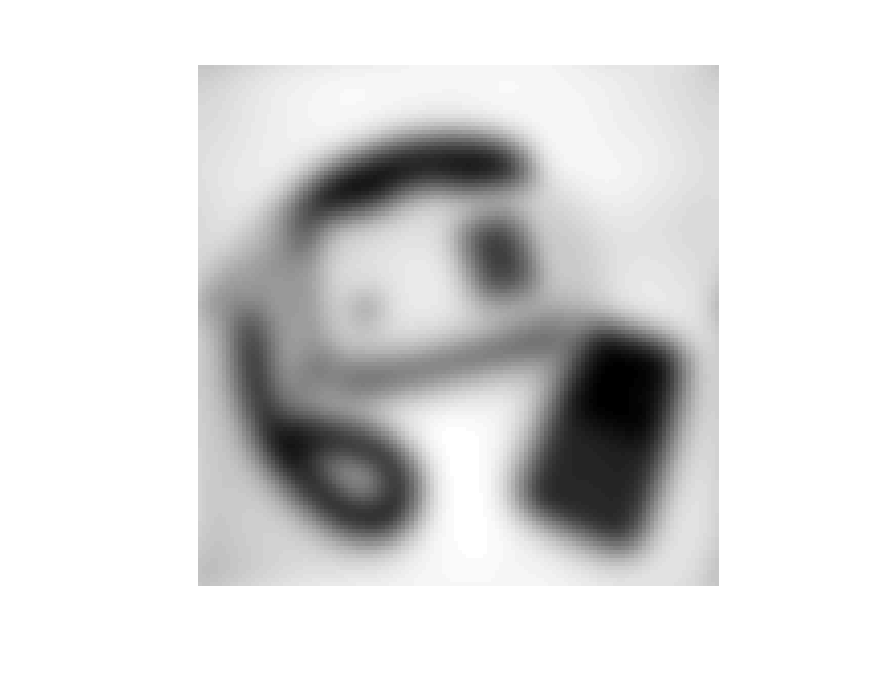
\includegraphics[scale=0.5]{./images/Q16/phone_16.eps}
      \caption{The result of the application of a gaussian function with $t=16$ to image \texttt{phonecalc128}.}
      \label{fig:Q16_phone_16}
    \end{figure}
  \end{minipage}
  \hspace{0.05\linewidth}
  \begin{minipage}{0.25\linewidth}
    \begin{figure}[H]
      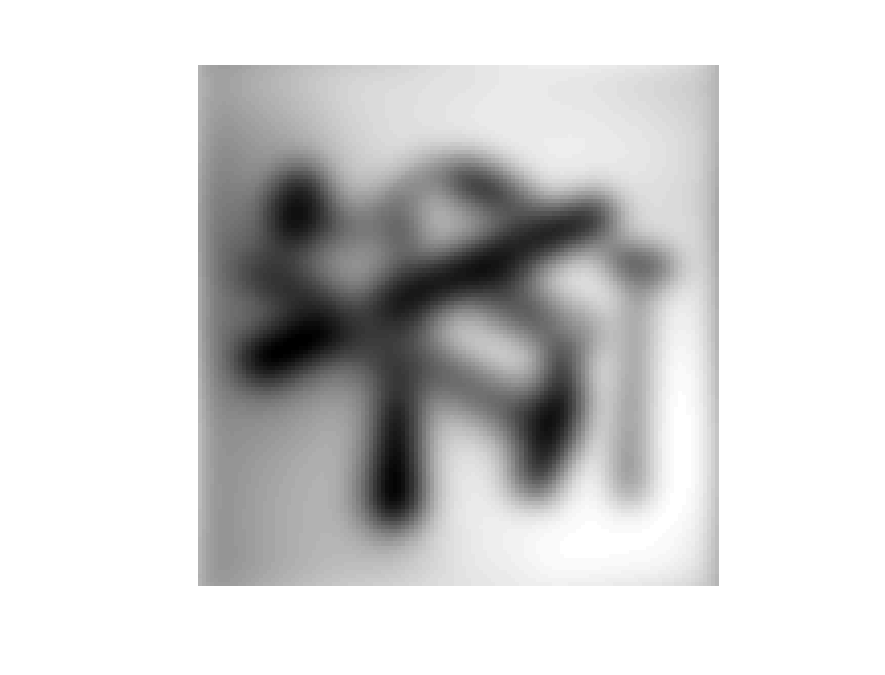
\includegraphics[scale=0.5]{./images/Q16/few_16.eps}
      \caption{The result of the application of a gaussian function with $t=16$ to image \texttt{few128}.}
      \label{fig:Q16_few_16}
    \end{figure}
  \end{minipage}
    \hspace{0.05\linewidth}
  \begin{minipage}{0.25\linewidth}
    \begin{figure}[H]
      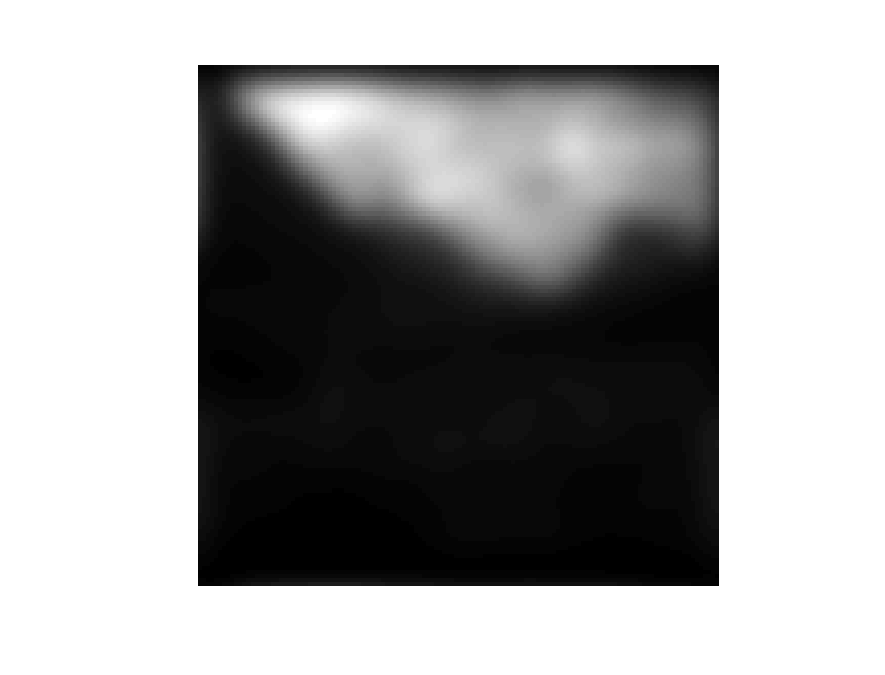
\includegraphics[scale=0.5]{./images/Q16/nallo_16.eps}
      \caption{The result of the application of a gaussian function with $t=16$ to image \texttt{nallo128}.}
      \label{fig:Q16_nallo_16}
    \end{figure}
  \end{minipage}
\end{minipage}
\\


\begin{minipage}{\linewidth}
  \begin{minipage}{0.25\linewidth}
    \begin{figure}[H]
      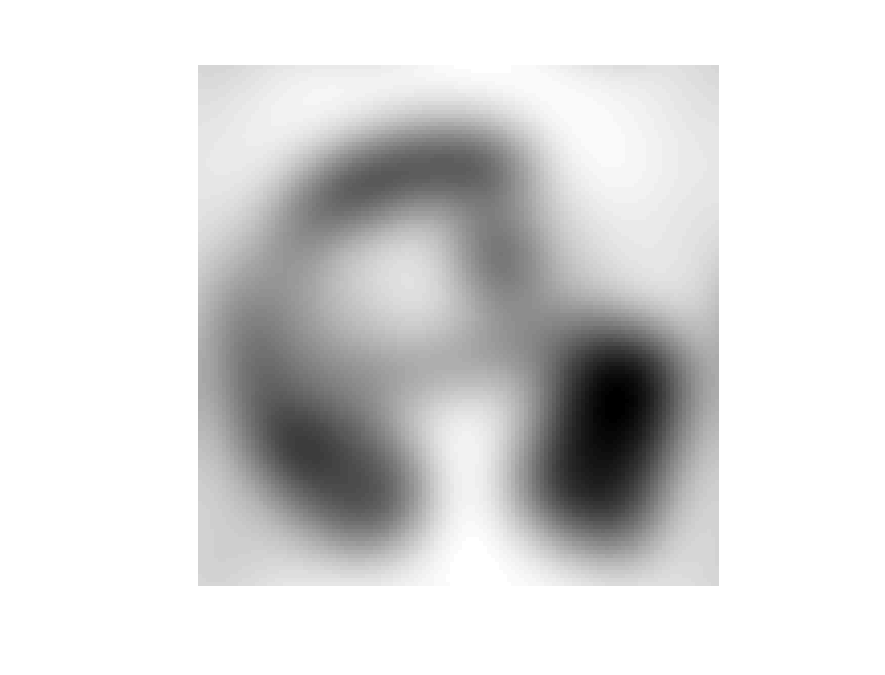
\includegraphics[scale=0.5]{./images/Q16/phone_64.eps}
      \caption{The result of the application of a gaussian function with $t=64$ to image \texttt{phonecalc128}.}
      \label{fig:Q16_phone_64}
    \end{figure}
  \end{minipage}
  \hspace{0.05\linewidth}
  \begin{minipage}{0.25\linewidth}
    \begin{figure}[H]
      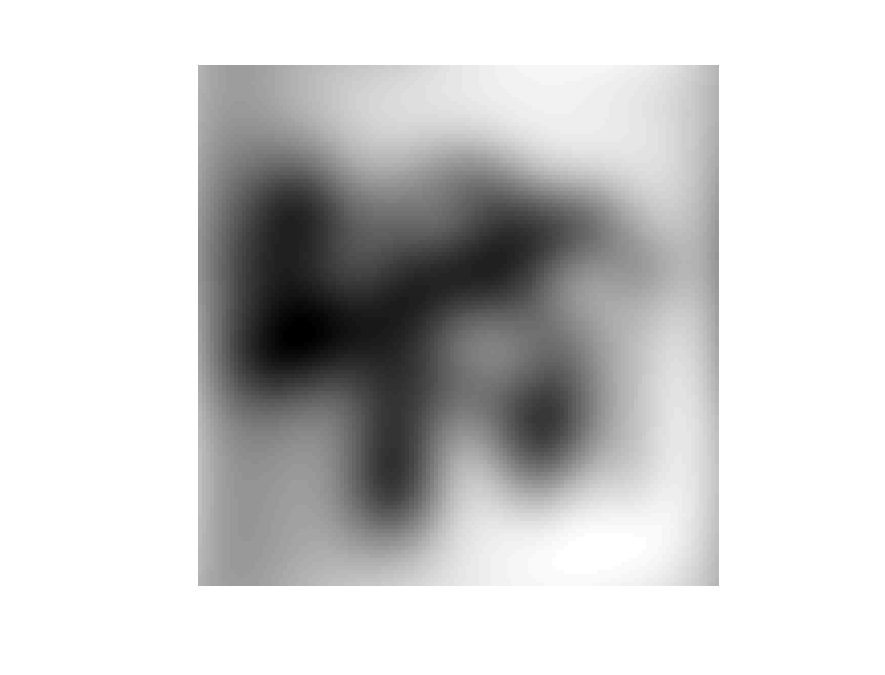
\includegraphics[scale=0.5]{./images/Q16/few_64.eps}
      \caption{The result of the application of a gaussian function with $t=64$ to image \texttt{few128}.}
      \label{fig:Q16_few_64}
    \end{figure}
  \end{minipage}
    \hspace{0.05\linewidth}
  \begin{minipage}{0.25\linewidth}
    \begin{figure}[H]
      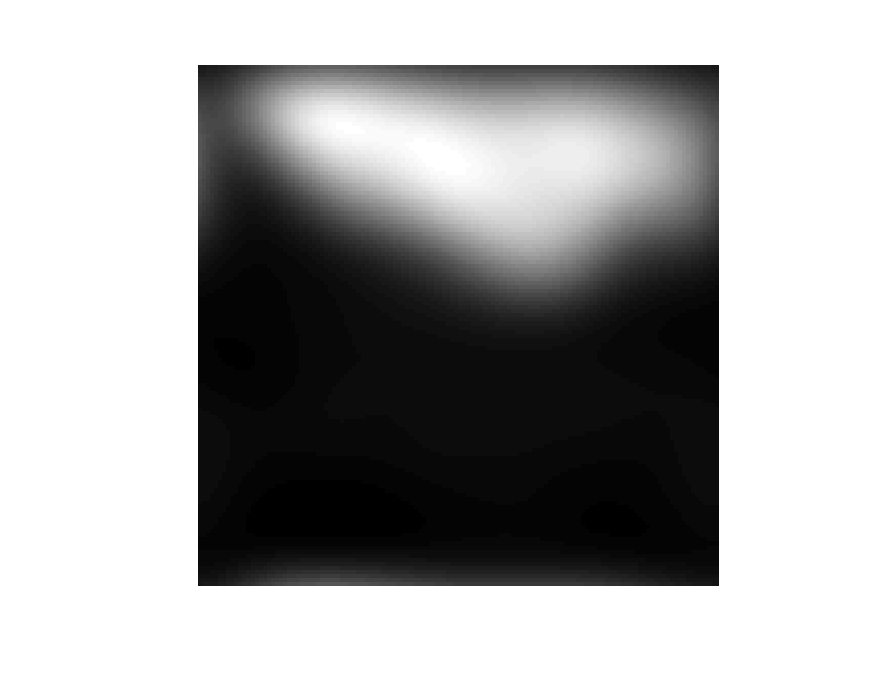
\includegraphics[scale=0.5]{./images/Q16/nallo_64.eps}
      \caption{The result of the application of a gaussian function with $t=64$ to image \texttt{nallo128}.}
      \label{fig:Q16_nallo_64}
    \end{figure}
  \end{minipage}
\end{minipage}
\\



\begin{minipage}{\linewidth}
  \begin{minipage}{0.25\linewidth}
    \begin{figure}[H]
      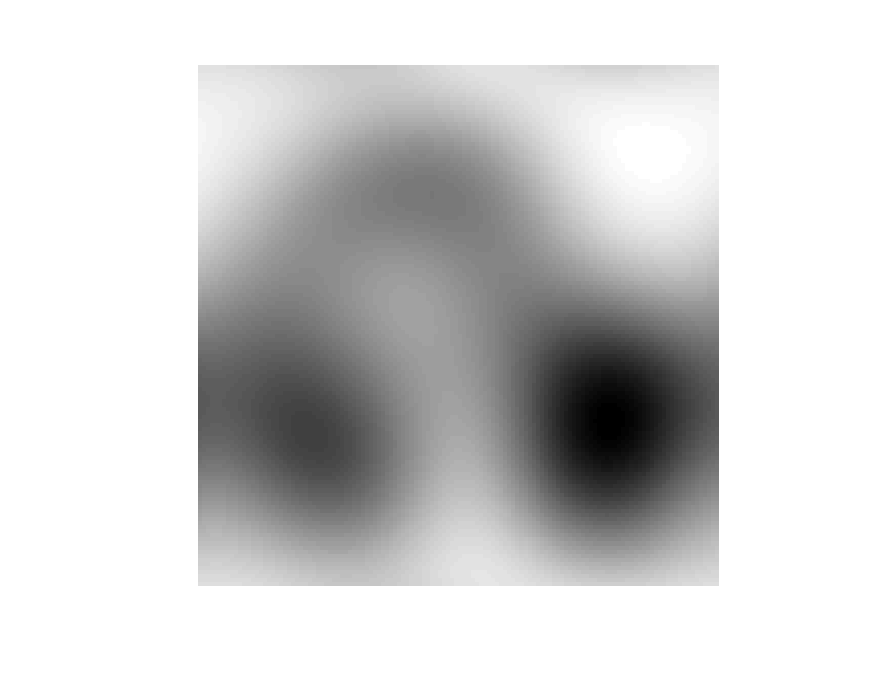
\includegraphics[scale=0.5]{./images/Q16/phone_256.eps}
      \caption{The result of the application of a gaussian function with $t=256$ to image \texttt{phonecalc128}.}
      \label{fig:Q16_phone_256}
    \end{figure}
  \end{minipage}
  \hspace{0.05\linewidth}
  \begin{minipage}{0.25\linewidth}
    \begin{figure}[H]
      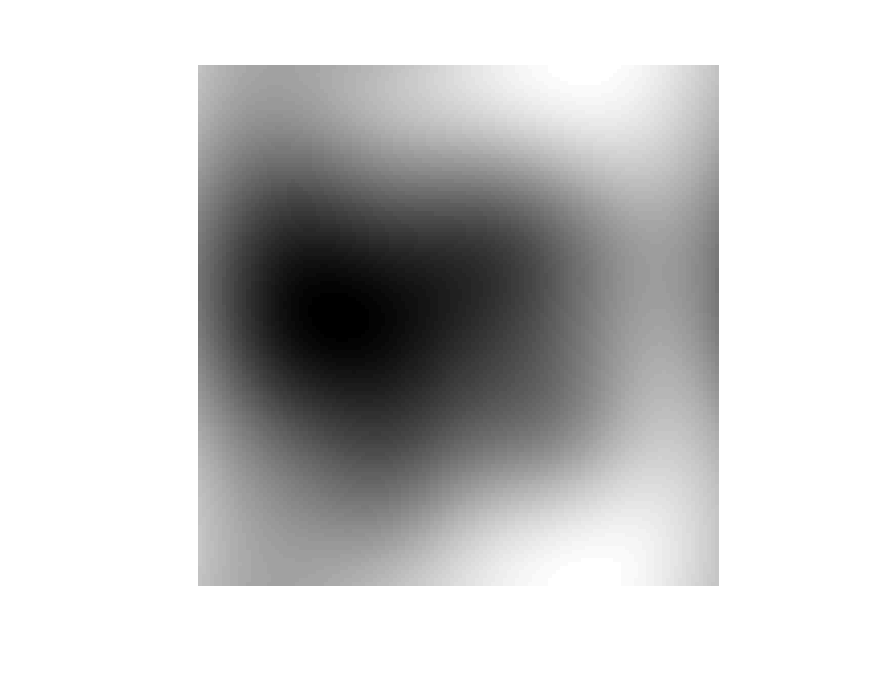
\includegraphics[scale=0.5]{./images/Q16/few_256.eps}
      \caption{The result of the application of a gaussian function with $t=256$ to image \texttt{few128}.}
      \label{fig:Q16_few_256}
    \end{figure}
  \end{minipage}
    \hspace{0.05\linewidth}
  \begin{minipage}{0.25\linewidth}
    \begin{figure}[H]
      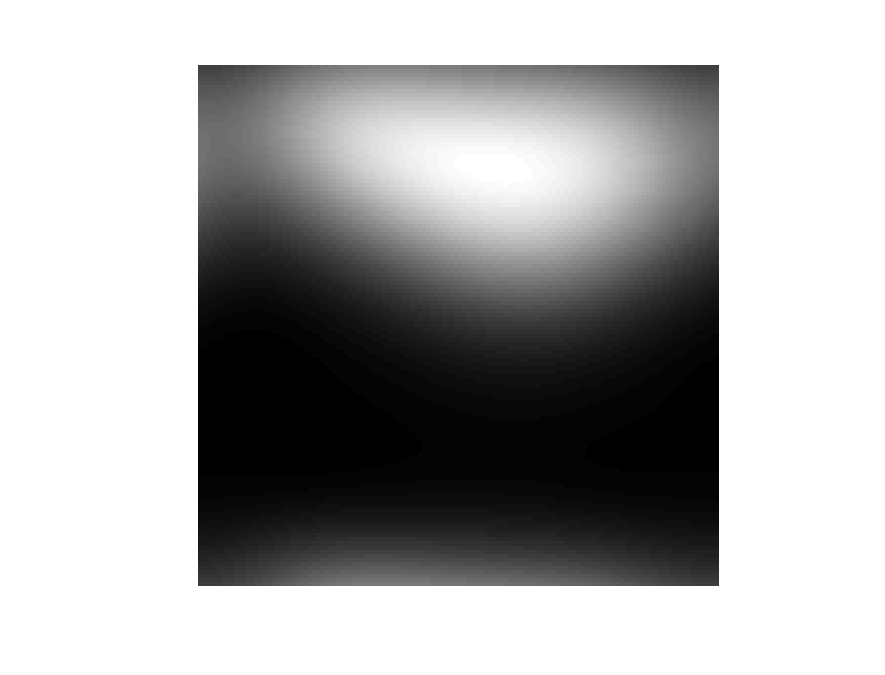
\includegraphics[scale=0.5]{./images/Q16/nallo_256.eps}
      \caption{The result of the application of a gaussian function with $t=256$ to image \texttt{nallo128}.}
      \label{fig:Q16_nallo_256}
    \end{figure}
  \end{minipage}
\end{minipage}
\\


The thing to notice here is that the higher the value of $t$, the more blurry the output image is.
This is reasonable since the higher the variance used, the smaller the cut-off frequency is as examined in the two previous questions,
and the more restricted the band of frequencies is toward the lower frequencies.
Hence, as $t$ increases, the less details, that is, regions of higher frequencies, are preserved. 